\section{Research}

\subsection{July 13 Distance between Bad Cone at a Cube to the Cube}

\begin{figure}[H]
    \centering
    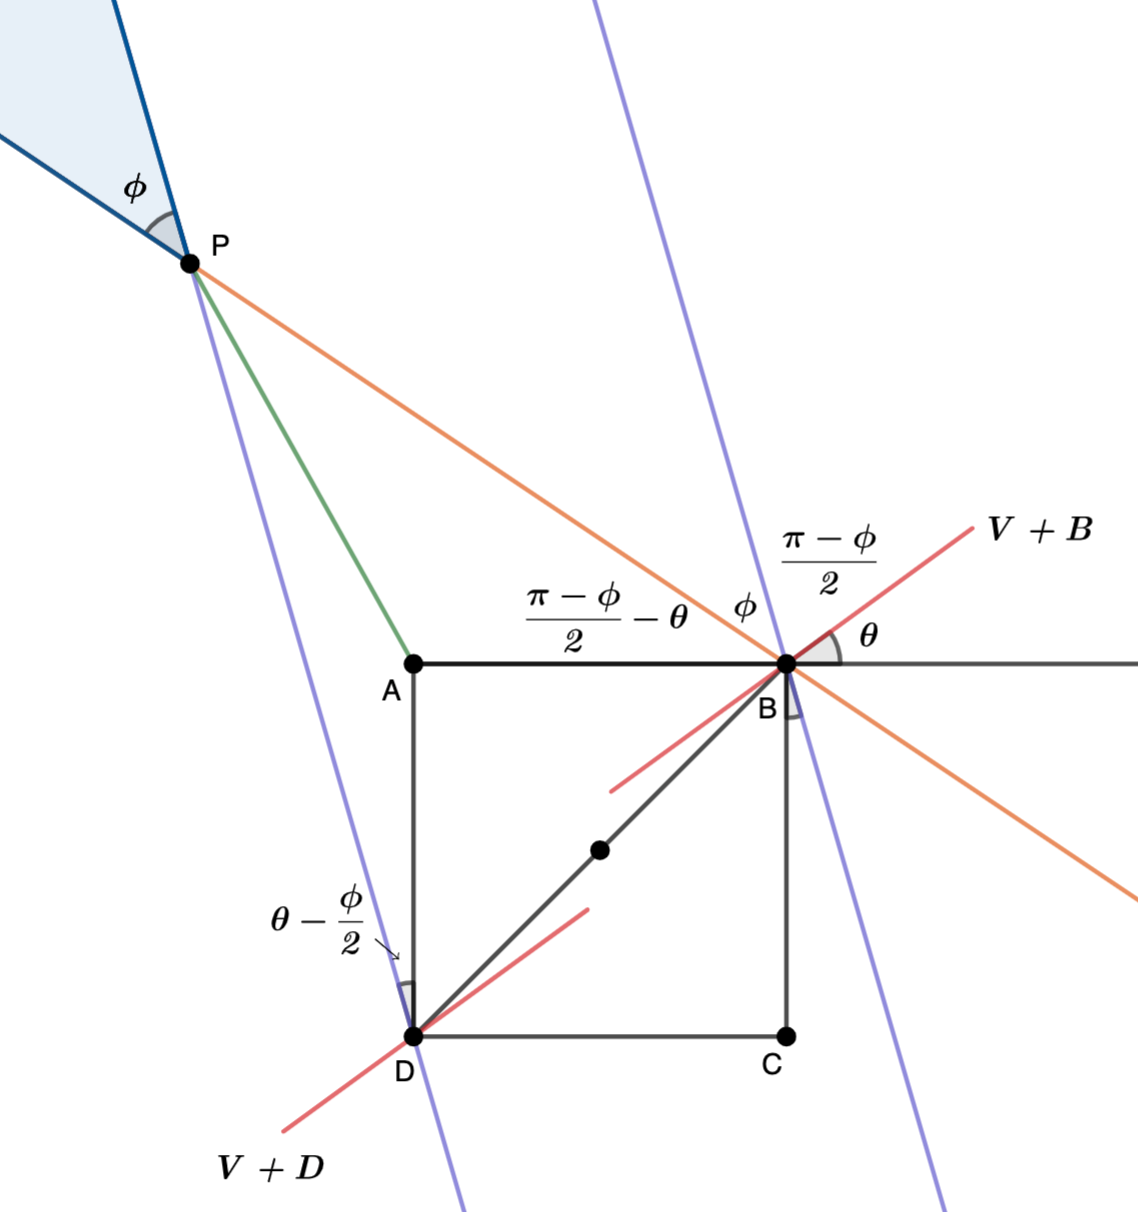
\includegraphics[width=.66\textwidth]{images/dist-CBQ2Q.png}
\end{figure}

\begin{lemma}
    For a dyadic cube $Q\in \rr^2$, $V\in G(1,2)$, $\alpha\in(0,1)$, assume that the inclination angle of $V$ is $\theta$, then $\dist(C_\calB^2(Q, V, \alpha), Q) = s\cdot \side Q$ where $s$ is
    \begin{equation*}
        \sqrt{ \left(\alpha + \sqrt{1-\alpha^2} \right)|\cos \theta-\sin\theta| \left(  \frac{\left(\alpha + \sqrt{1-\alpha^2} \right)|\cos \theta-\sin\theta|}{4\alpha^2(1-\alpha^2)} - \frac{\sin\theta}{\alpha} -\frac{\cos\theta}{\sqrt{1-\alpha^2}}  \right) + 1}
    \end{equation*}
    and $\dist(C_\calB^2(Q, V, \alpha), \centerof Q) = s^\prime \cdot \side Q$ where $s^\prime$ is 
    \begin{equation*}
        \sqrt{ \left(\alpha + \sqrt{1-\alpha^2} \right)|\cos \theta-\sin\theta|\left( \frac{\left(\alpha + \sqrt{1-\alpha^2} \right)|\cos \theta-\sin\theta|}{4\alpha^2(1-\alpha^2)} - \frac{\cos\theta + \sin\theta}{2\alpha} - \frac{\cos\theta-\sin\theta}{2\sqrt{1-\alpha^2}}  \right) + \frac{1}{2}}
    \end{equation*}
\end{lemma}
\begin{proof}
    For convenience, assume that $A, B, C, D$ are four corners of $Q$(note that point $A, B, C\notin Q$, but exist in the cube system and $\partial Q$), $P$ is one of vertices of $C_\calB^2(Q, V, \alpha)$, $\phi$ is the aperture of $Q_\calB^2(Q, V, \alpha)$. Then for any $y\in\partial C_\calB(B, V, \alpha)$, $\dist(y-B, V) = \alpha|y-B| = \sin\frac{\pi-\phi}{2} |y-B|$, so $\phi = \pi-2\arcsin \alpha$. Note that $\angle PBA = (\pi-\phi)/2 -\theta = \arcsin \alpha -\theta$, $\angle PDA = \pi/2 - ((\pi-\phi)/2 - \theta) - \phi = \theta -\phi/2 = \theta + \arcsin \alpha -\pi/2$. By the \textit{Law of Sines},
    \begin{equation*}
        \begin{split}
            |P-D| &= \frac{|B-D|}{\sin \angle BPD}\cdot \sin\angle PBD \\
            &= \frac{ \sqrt{2}\sin(\arcsin (\alpha) - \theta + \pi/4)}{\sin (2\arcsin \alpha) } \cdot \side Q\\
            &= \frac{ \left(\alpha + \sqrt{1-\alpha^2} \right)|\cos \theta-\sin\theta|}{2\alpha\sqrt{1-\alpha^2} } \cdot \side Q
        \end{split}
    \end{equation*} 
    Then applying the \textit{Law of Cosines}, denoting $|P-D|$ as $t\cdot \side Q$,
    \begin{equation*}
        \begin{split}
            \dist(C_\calB^2(Q, V, \alpha), Q) &= |P-A|\\
            &= \sqrt{|P-D|^2 + |A-D|^2 - 2|P-D||A-D|\cos \angle ADP} \\
            &= \sqrt{t^2 + 1 - 2t\cdot\cos(\theta + \arcsin \alpha -\pi/2) }\cdot \side Q \\
            &= \sqrt{t^2 + 1 - 2t\left( \sqrt{1-\alpha^2} \sin \theta + \alpha\cos\theta\right) }\cdot \side Q \\
            &= s\cdot \side Q
        \end{split}
    \end{equation*}
    Similarly,
    \begin{equation*}
        \begin{split}
             \dist(C_\calB^2(Q, V, \alpha), Q), \centerof Q) &= |P- \centerof Q| \\
            &= \sqrt{\frac{1}{4}|B-D|^2 + |P-D|^2 - |B-D||P-D|\cos\angle PDB} \\ 
            &= \sqrt{\frac{1}{2} + t^2 - \sqrt{2} t \cos(\theta + \arcsin \alpha -\pi/4)}\cdot \side Q \\
            &= \sqrt{\frac{1}{2} + t^2 -  t \left( \sqrt{1-\alpha^2}(\cos\theta +\sin\theta) + \alpha(\cos\theta -\sin\theta)\right)}\cdot \side Q \\
            &= s^\prime \cdot \side Q
        \end{split}
    \end{equation*}
\end{proof}

\newpage
\subsection{July 8 Complete and Modify our Lemma}

\begin{corollary}[{\cite[Corollary 7.1]{naples2020}}]\label{LisaCoro7.1}
    Let $\mu$ be a Radon measure on $H, V$ be an $m$-dimensional linear plane in $H$, $\alpha \in(0,1)$, and $0<r<\infty$. If for $\mu$-a.e. $x \in H$
    $$
    \mu\left(C_{\mathcal{B}}(x, r, V, \alpha)\right)=0
    $$
    then $\mu$ is carried by $m$-Lipschitz graphs.
\end{corollary}



\begin{lemma}\label{lemma:s-guarantee-containQ-between-2alpha}
    For $0<\alpha_2<\alpha_1<1$, $V\in G(1, 2)$, a dyadic cube $Q$ in $\rr^2$, and $s\geq \frac{3\sqrt{2}(1+\alpha_2)}{\alpha_1-\alpha_2}$, a dilation cube $2R$ such that $R$ is the dyadic cube with the same side length as $Q$ and
    \begin{equation*}
        \dist(Q, 2R)\geq s\cdot \side Q
    \end{equation*}
    then
    \begin{enumerate}[(i)]
        \item \label{lemma-1:s-guarantee-containQ-between-2alpha} {\color{red} if $2R\subset C_\calB^{2,1}(Q, V, \alpha_1)$, then $2R\subset  C_\calB^{2,2}(Q, V, \alpha_2)$.}
        \item \label{lemma-2:s-guarantee-containQ-between-2alpha} if for $n = n(s) \in \nn$ such that $2^n\geq 2(\sqrt{2}+1)s + 3\sqrt{2}$, then $2sQ\subset 2^n R $.
        \item \label{lemma-3:s-guarantee-containQ-between-2alpha} if for $m = m(s) \in \nn$ such that $2^m \geq (3\sqrt{2}+2)s + 3\sqrt{2}$, then $3sQ\subset 2^m R$. 
    \end{enumerate}
\end{lemma}
\begin{proof}
    \begin{enumerate}[(i)]
        \item When {\color{red}$2R\subset C_\calB^{2,1}(Q, V, \alpha_1)$}, there exists some $r\in 2R\cap C_\calB^1(Q, V, \alpha_1)$ and hence {\color{red} for any} $q\in Q$ such that $r\in C_\calB(q, V, \alpha_1)$, so $\dist(r-q, V)>\alpha_1|r-q|$. Besides, {\color{red}arbitrary} $r^\prime\in 2R$ and $q^\prime\in Q$ must satisfy $|r-r^\prime|\leq 2\sqrt{2}\cdot\side R$ and $|q-q^\prime|\leq \sqrt{2}\cdot\side Q$, respectively. Assume that $|r-q| = s^\prime\cdot\side Q$ then $s^\prime \geq s$. Since $ |r-r^\prime| \geq|\dist (r^\prime-q^\prime, V)-\dist(r-q, V)| - |q-q^\prime|$, no matter $\dist (r^\prime-q^\prime, V)\leq \dist(r-q, V)$ or $\dist (r^\prime-q^\prime, V)\geq \dist(r-q, V)$,

        \begin{align*}
            \dist(r^\prime-q^\prime, V) &\geq \dist(r-q, V)-|q-q^\prime|-|r-r^\prime| \\
            &> \alpha_1|r-q| - 3\sqrt{2} \cdot\side Q\\
            &\geq (\alpha_1 s^\prime- 3\sqrt{2})\cdot\side Q\\
            &\geq \alpha_2(s^\prime+3\sqrt{2})\cdot\side Q  &&(s^\prime \geq s \geq \frac{3\sqrt{2}(1+\alpha_2)}{\alpha_1-\alpha_2}) \\
            &\geq \alpha_2(|r-q|+|r-r^\prime|+|q-q^\prime|)\\
            &\geq \alpha_2|r^\prime-q^\prime|
        \end{align*}

        Therefore, {\color{red}$2R\subset \{R: R\subset \bigcap_{q^\prime\in Q} C_\calB(q^\prime, V, \alpha)\} =  C_\calB^{2,2}(Q, V, \alpha_2)$.}
        \item Assume for all $q^{\prime\prime}\in 2sQ$, then
        \begin{equation*}
            \begin{split}
                |\centerof 2R - q^{\prime\prime}| &\leq \left(\frac{1}{2}\diam 2R + \dist(2R, Q) + \frac{1}{2}\diam Q + \frac{1}{2}\diam 2sQ\right)\\
                &\leq (\sqrt{2}+s+\frac{\sqrt{2}}{2} + \sqrt{2}s ) \side Q \\
                &\leq \frac{2^n}{2}\side R = \frac{1}{2}\side 2^n R
            \end{split}
        \end{equation*}
        which implies that $\displaystyle 2sQ \subset B(\centerof R, \frac{1}{2}\side 2^n R)\subset 2^n R$.
        \item Similarly, assume $\forall q^{\prime\prime\prime}\in 3sQ$, then
        \begin{equation*}
            \begin{split}
                |\centerof 2R - q^{\prime\prime\prime}| &\leq (\frac{1}{2}\diam 2R + \dist(2R, Q) + \frac{1}{2}\diam Q + \frac{1}{2}\diam 3sQ)\\
                &\leq (\sqrt{2}+s+\frac{\sqrt{2}}{2} + \frac{3}{2}\sqrt{2}s ) \side Q \\
                &\leq \frac{2^m}{2}\side R = \frac{1}{2}\side 2^m R
            \end{split}
        \end{equation*}
        which implies that $\displaystyle 3sQ \subset B(\centerof R, \frac{1}{2}\side 2^m R)\subset 2^m R$.
    \end{enumerate}
\end{proof}


\begin{lemma}\label{lemma:doubling-meaure-4cubes}
    If there exist $K\geq1$, such that for $\mu$-a.e. $x\in \rr^2, 0<r<\infty$, 
    \begin{equation}\label{eq:doubling}
        \mu(B(x, 2r))\leq K\mu(B(x,r))
    \end{equation} 
    then for any dyadic cube $Q$ containing $x$ where (\ref{eq:doubling}) holds, {\color{red}$s, n\in \nn, n\geq 2$, $s\in \nn$
    \begin{equation}\label{eq:doubling4cubes}
        \mu(2^n sQ)\leq K^{3n-3} \mu(2sQ)
    \end{equation}}
\end{lemma}
\begin{proof}
    By the half open definition of the dyadic cube, for $\mu$-a.e. $x\in \rr^2$, $x$ must be in only one cube $Q$. Let {\color{red}$r = s\cdot \side Q /2$. We claim that $2^n sQ\subset B(x, 2^{3n-3}r)$ and $B(x, r)\subset 2sQ$. For any $q\in 2^n sQ$, $|\centerof Q -x|\leq \sqrt{2}/2\cdot\side Q $ and $|\centerof 2^n sQ -q|\leq \sqrt{2}/2 \cdot\side 2^n sQ  = 2^{n-1}\sqrt{2}s\cdot \side Q$. Note that $n\geq 2$, so
    \begin{equation*}
        |x-q| \leq \left(\frac{\sqrt{2}}{2} + 2^{n-1}\sqrt{2}s \right) \side Q < \frac{2^{3n-3} s}{2} \side Q = 2^{3n-3}r
    \end{equation*}
Then $q\in B(x, 2^{3n-3}r)$ and thus $2^n sQ\subset B(x, 2^{3n-3}r)$. Consider that for all $p\in \bigcup_{q\in Q} B(q, r)\setminus sQ$, $\dist(p, \partial sQ)\leq r = \dist(\partial 2sQ, sQ)$, so $B(x, r)\subset \bigcup_{q\in Q} B(q, r)\subset 2sQ$. Therefore, by the containments and (\ref{eq:doubling}), 
    \begin{equation*}
        \mu(2^n sQ) \leq \mu(B(x, 2^{3n-3}r)) \leq \prod_{i=1}^{3n-3} K \cdot \mu(B(x,r))\leq K^{3n-3}\mu(B(x,r))\leq K^{3n-3}\mu(2sQ)
    \end{equation*}
    }
\end{proof}
    

\begin{lemma}\label{lemma:limQ-2sQ-0}
    Let $\mu$ be a measure on $\rr^2$ and $E$ denote the set of points $\mu$-a.e. $x\in\rr^2$.For $x\in E$, there exists $K\geq 1$ such that $\mu(B(x, 2r))\leq K\mu(B(x,r))$. For $0<\alpha_2<\alpha_1<1$, $V\in G(1,2)$, any dyadic cube $Q_k$ contained $\mu$-a.e. $x$ in $E$ with the side length $2^{-k}, k\in\nn$, and a dilation constant $s\in\nn$ such that $s \geq \frac{6\sqrt{2}(1+\alpha_2)}{\alpha_1-\alpha_2}$, when $Q\downarrow x$ (i.e. $k\rightarrow\infty \Rightarrow 2^{-k}\downarrow 0$),
    {\color{red}
    \begin{equation}\label{eq:limBC-2sQ-0}
        \frac{\mu(C_\calB^{2,1}(Q_k, V, \alpha_2)\cap 2sQ_k)}{\mu(2sQ_k)} \rightarrow 0
    \end{equation}
    }
    if and only if $E$ is $\mu$-carried by Lipschitz graphs {\color{red}with respect to $V$ and the Lipschitz constant at most $\sqrt{\alpha_2^2/(1-\alpha_2^2)}$}
\end{lemma}
\begin{proof}
    We first show the sufficient condition holds. By (\ref{eq:limBC-2sQ-0}) there exists a large enough $k$ such that for any $\delta>0$,
    {\color{red}
    \begin{equation}\label{eq:delta-4-limQ-2sQ-0}
        \mu(C_\calB^{2,1}(Q_k, V, \alpha_2)\cap 2sQ) < \delta\mu(2sQ_k)
    \end{equation}
    }
    Fix a $k$ and $Q_k\ni x$. Now construct sets:
    {\color{red}
    \begin{equation*}
        \begin{split}
            S_{Q_k} &:= \{2R_k: \dist(2R_k, Q_k)\geq \frac{1}{2}s\cdot\side Q_k, 2R_k\cap(2sQ_k\cap C_\calB^{2, 1} (Q_k, V, \alpha_1))\neq \emptyset\} \\
            S_{Q_k}^\prime &:= \{2R_k: \dist(2R_k, Q_k)\geq \frac{1}{2}s\cdot\side Q_k, 2R_k\subset 2sQ_k\cap C_\calB^{2, 1} (Q_k, V, \alpha_1)\} \\
            S_{Q_k}^{\prime\prime} &:= S_{Q_k} \setminus S_{Q_k}^\prime
        \end{split}
    \end{equation*}
    }
    where $2R_k$ is the dilation cube of the dyadic cube $R_k$ with the same side length as $Q_k$. Then for any $2R_k\in S_{Q_k}^\prime$, by Lemma \ref{lemma:s-guarantee-containQ-between-2alpha} (\ref{lemma-1:s-guarantee-containQ-between-2alpha}), $2R_k\subset  C_\calB^{2,2}(Q_k, V, \alpha_2)$ and apparently $2R_k\subset  C_\calB^{2,1}(Q_k, V, \alpha_2)\cap 2sQ_k$ as well{\color{red} ($2R_k\subset  C_\calB^{2}(Q_k, V, \alpha_2)\cap 2sQ_k$, too)}. Then, fix $2^n=n(s), n\in\nn$ such that $2^n\geq (\sqrt{2}+1)s + 3\sqrt{2}$, then by Lemma \ref{lemma:s-guarantee-containQ-between-2alpha} (\ref{lemma-2:s-guarantee-containQ-between-2alpha}), $2sQ_k\subset 2^n R_k$. Now assume that there are some $\mu$-a.e. $x$ are contained in $2R_k$, then by (\ref{eq:delta-4-limQ-2sQ-0}) and Lemma \ref{lemma:doubling-meaure-4cubes} (\ref{eq:doubling4cubes}), 
    \begin{equation*}
        \mu(2^n R_k)\leq K^{3n-3}\mu(2R_k)\leq K^{3n-3}\mu(C_\calB^{2,1}(Q, V, \alpha_2)\cap 2sQ_k) < \delta K^{3n-3} \mu(2sQ_k)
    \end{equation*}
    which is a contradiction if we choose $\delta<K^{-3n+3}$. Thus, 
    \begin{equation*}
        \mu(S_{Q_k}^\prime) = \mu(\bigcup_{2R_k\in S_{Q_k}^\prime} 2R_k)=\sum_{2R_K \in S^\prime_{Q_k}}\mu(2R_k)=0
    \end{equation*}
    Similarly, we will consider any $2R_k^\prime\in S^{\prime\prime}_{Q_k}$. Now fix $2^m = m(s), m\in\nn$ such that $2^m \geq (3\sqrt{2}/2+1)s + 3\sqrt{2}$ and then by Lemma \ref{lemma:s-guarantee-containQ-between-2alpha} (\ref{lemma-2:s-guarantee-containQ-between-2alpha}), $2R_k^\prime \subset  3sQ_k \subset 2^m R_k$. Then with the similar contradiction proof noting that $\mu(2sQ_k)\leq \mu(3sQ_k)$, we can say $\mu(S_{Q_k}^{\prime\prime})=0$. Hence, $\mu(S_{Q_k}) = \mu(S_{Q_k}^\prime \cup S_{Q_k}^{\prime\prime}) = 0$. {\color{red}Note that this will hold for all dyadic cubes with the smaller side length than $Q_k$.}
    
    {\color{red}Assume that $r= (s-\sqrt{2}/2)\cdot \side Q_k$ then for $\mu$-a.e. $x\in Q_k$, any $y\in C_\calB(x,r, V, \alpha_1)$, we have $\dist(x-y,V)>\alpha_1|x-y|$. Choose $k^\prime > k$, and then there exists dyadic cube $Q_{k^\prime}\ni x$ such that $(\sqrt{2}+s/2)\cdot 2^{-k^\prime} \leq |y-x|$. Then $\dist(y, Q_{k^\prime})|\geq |y-x|-\dist(x, \partial Q_{k^\prime})\geq (\sqrt{2} +s/2-\sqrt{2})\side Q_{k^\prime} = s/2\cdot\side Q_{k^\prime}$, so that $y\in \bigcup_{i=k}^\infty \{S_{Q_i}: x\in Q_i\subset Q_k\}$.}
    Hence, $C_\calB(x, r, V, \alpha_1)\subset \bigcup_{i=k}^\infty \{S_{Q_i}: x\in Q_i\subset Q_k\}$. Thus, for $\mu$-a.e. $x\in E$ where $x$ must be contained in only one $Q_k$,
    \begin{equation*}
        \begin{split}
            \mu(C_\calB(x, r, V, \alpha_1))\leq \mu\left( \bigcup_{i=k}^\infty \left\{S_{Q_i}:x\in Q_i\subset Q_k \right)\}\right) = 0
        \end{split}
    \end{equation*}
    It follows immediately that for $\mu$-a.e. $x\in E$, $\mu(C_\calB(x, r, V, \alpha_1)) = 0$. Applying Corollary \ref{LisaCoro7.1}, the sufficient condition holds then.

    {\color{red}
    To prove the necessary condition, suppose that $E$ is contained in a collection of Lipschitz graphs $\{\Gamma_i\}$ where $\Gamma_i\cap E = \{(v, f_i(v)) : (v, f_i(v))\in E\}\subset V\times V^\perp = \rr^2$ where $f_i$ is a Lipschitz function $f_i: V\rightarrow V^\perp$ with Lipschitz constant $L_i$ at most $\sqrt{\alpha_2^2/(1-\alpha_2^2)}$. Let any point $p = (v_1, f_i(v_1)), q = (v_2, f_i(v_2))\in E\cap \Gamma_i$, then we have $|f_i(v_1)-f_i(v_2)| \leq L_i |v_1- v_2|$. Consider the good cone $C_\calG(p, V, \alpha_2)$, then, 
    \begin{align*}
        |p-q| = \sqrt{|v_1-v_2|^2 + |f_i(v_1) - f_i(v_2)|^2} 
        \geq \sqrt{\frac{1}{L_i^2} + 1} |f_i(v_1) - f_i(v_2)|  
        \geq \frac{1}{\alpha_2} \dist(p-q, V)
    \end{align*}
    Thus, $q\in C_\calG(p, V, \alpha_2)$. As $p,q, \Gamma_i$ arbitrary, $E\subset C_\calG(x, V, \alpha_2), \forall x\in E$. Now, for $Q_k\ni x$,
    \begin{equation}\label{containment-necessary-condition}
        C_\calB^{2}(Q_k, V, \alpha_2)\cap 2sQ_k \subset C_\calB(x,V, \alpha_2) \cap 2sQ_k \subset 2sQ_k \setminus C_\calG(x, V, \alpha_2) \subset 2sQ_k \setminus E   
    \end{equation}
    Next, we claim that
    \begin{equation}\label{eq:muE/2sQ-/-mu2sQ-0}
        \lim_{k\rightarrow \infty}\frac{\mu(2sQ_k \setminus E)}{\mu(2sQ_k)} =0
    \end{equation}
    We choose $r_k = (\sqrt{2}s + \sqrt{2}/2) \cdot 2^{-k}$ such that apparently $2sQ_k\subset B(x,r_k)\subset 4sQ_k$ for any $x\in Q_k$. Note that by our choice of $r_k$, when $k\rightarrow\infty$, then $r_k\rightarrow 0$. By Lemma \ref{lemma:doubling-meaure-4cubes} and Lemma \ref{coro:mattila-coro-2.14},
    \begin{equation*}
        \begin{split}
            \lim_{k\rightarrow \infty} \frac{\mu(2sQ_k \setminus E)}{\mu(2sQ_k)} 
            \leq \lim_{k\rightarrow \infty} \frac{\mu(2sQ_k \setminus E)}{K^{-3}\mu(4sQ_k)} 
            \leq K^3 \lim_{k\rightarrow \infty} \frac{\mu(B(x, r_k) \setminus E)}{\mu(B(x, r_k))} = 
            0
        \end{split}
    \end{equation*}
    Therefore (\ref{eq:muE/2sQ-/-mu2sQ-0}) holds. Combining (\ref{containment-necessary-condition}),
    \begin{equation*}
        \lim_{k\rightarrow \infty}\frac{\mu(C_\calB^{2}(Q_k, V, \alpha_2)\cap 2sQ_k)}{\mu(2sQ_k)} =0
    \end{equation*}
    This completes the proof of the necessary condition. 
    }
\end{proof}




\newpage
\subsection{July 7 Complete Necessary Condition for the Lemma}
\begin{lemma}[Sufficient Condition for Geometric Lemma]\label{lemma:Suf-4-Geo-Lemma} Let $V\in G(1,2)$, $\alpha\in(0,1)$, non-empty set $E\subset \rr^2$. If there exists a Lipschitz function $f: V\rightarrow V^\perp$ with Lipschitz constant at most $\alpha$, such that $E$ is contained in the Lipschitz graph $\Gamma = \{(x, f(x)) : x\in V\}\subset V\times V^\perp = \rr^2$, then $E\subset C_\calG(p, V, \alpha), \forall p\in E$.
\end{lemma}
\begin{proof}
    Assume the Lipschitz constant is $L\leq \alpha$. Let any point $p = (x_1, f(x_1)), q = (x_2, f(x_2))\in E\subset \Gamma$, then we have $|f(x_1)-f(x_2)| \leq L |x_1- x_2|$. Consider the good cone $C_\calG(p, V, \alpha)$. Then, 
    \begin{equation*}
            \dist(p-q, V) = |f(x_1)- f(x_2)| 
            \leq L|x_1-x_2| 
            \leq \alpha \sqrt{|x_1-x_2|^2 + |f(x_1)-f(x_2)|^2}
            = \alpha |p-q|
    \end{equation*}
    Thus, $q\in C_\calG(p, V, \alpha)$. As $p,q$ arbitrary, $E\subset C_\calG(p, V, \alpha), \forall p\in E$
\end{proof}

\begin{lemma}\label{lemma:limmuE/2sQ-/-mu2sQ-0}
    Let $\mu$ be a Radon measure on $\rr^2$ and $E\subset \rr^2$ measurable. For $x\in E$, there exists $K\geq 1$ such that $\mu(B(x, 2r))\leq K\mu(B(x,r))$. For any dyadic cube $Q_k$ with side length $2^{-k}$ contained $\mu$-a.e. $x\in E$, $s>3\sqrt{2}$(this is just simply set for this proof)
    \begin{equation*}
        \lim_{k\rightarrow \infty}\frac{\mu(2sQ_k \setminus E)}{\mu(2sQ_k)} =0
    \end{equation*}
\end{lemma}
\begin{proof}
    We choose $r$ where $(\sqrt{2}s + \sqrt{2}/2) \cdot 2^{-k} \leq r \leq (2\sqrt{2}s - \sqrt{2}/2)\cdot 2^{-k} $ such that $2sQ_k\subset B(x,r)\subset 4sQ_k$ for any $x\in Q_k$. Note that by our choice of $r$, when $k$ is large enough, $r < \epsilon, \forall \epsilon > 0$. Recall that by Lemma \ref{coro:mattila-coro-2.14}, for existed $\epsilon > 0$, whenever $r<\epsilon$, 
    \begin{equation}\label{eq:muE/B-/-muB-delta}
        \frac{\mu(E \setminus B(x, r))}{\mu(B(x, r))} < \frac{\delta}{K^3}, \quad \forall\delta > 0
    \end{equation}
    Besides, considering Lemma \ref{lemma:doubling-meaure-4cubes} and containment, and combining (\ref{eq:muE/B-/-muB-delta}), there exists a large enough $k$ such that 
    \begin{equation*}
        \frac{\mu(2sQ_k \setminus E)}{\mu(2sQ_k)}\leq \frac{\mu(2sQ_k \setminus E)}{K^{-3}\mu(4sQ_k)} \leq K^3 \frac{\mu(B(x, r) \setminus E)}{\mu(B(x, r))} < K^3\frac{\delta}{K^3} = \delta
    \end{equation*}
    Therefore the conclusion holds. 
\end{proof}

\textit{Alternative Proof.} In the fixed dyadic cube system, we can divide $E$ into countable many $E_i$ such that $\bigcup_i E_i = E$ and $E_i$ is contained in only one dilation cube $2sQ_{E_i, k}$ with $\side Q_{E_i, k} = 2^{-k}$($E_i$ may not be disjoint).  Define the Radon measure $\lambda_i$ by $\lambda_i(E_i) = \int_{E_i} \chi_{E_i} d \mu$ such that $\mu(E_i) = \lambda_i(E_i)$, $\mu(2sQ_{E_i, k}\setminus E_i) = \lambda_i(2sQ_{E_i, k}\setminus E_i) = 0$. Then $\lambda_i \ll \mu$ and by {\cite[Theorem 2.12(2)]{mattila1999geometry}}, considering $\mu$-a.e. $x\in E_i$
\begin{equation*}
    \int_{2sQ_{E_i, k}} D(\lambda_i, \mu, x)d\mu x = \lambda(2sQ_{E_i, k}) = \int_{2sQ_{E_i, k}} \chi_{E_i} d\mu
\end{equation*}
Hence, for any dyadic $Q_k$ conatined $x\in E$,
\begin{equation*}
    \begin{split}
        \lim_{k\rightarrow\infty} \frac{\mu(E\cap 2sQ_k)}{\mu(2sQ_k)} &=
        \lim_{k\rightarrow \infty} \frac{1}{\mu(2sQ_{E_i, k})}\int_{2sQ_{E_i, k}} \chi_{E_i} d\mu \\
        &= \lim_{k\rightarrow \infty} \frac{\lambda_i(2sQ_{E_i, k})}{\mu(2sQ_{E_i, k})} \\
        &= \lim_{k\rightarrow\infty} \frac{\lambda_i(E_i\cup (2sQ_{E_i,k}\setminus E_i))}{\mu(E_i\cup (2sQ_{E_i,k}\setminus E_i))} \\
        &= \lim_{k\rightarrow\infty} \frac{\lambda_i(E_i) +0}{\mu(E_i) +0} \\ 
        &= 1
    \end{split}
\end{equation*}
Therefore, 
\begin{equation*}
    \lim_{k\rightarrow\infty} \frac{\mu(2sQ_k\setminus E)}{\mu(2sQ_k)} = \lim_{k\rightarrow\infty} \frac{\mu(2sQ_k\setminus (2sQ_k\cap E))}{\mu(2sQ_k)} = \lim_{k\rightarrow\infty} \frac{\mu(2sQ_k)-\mu(2sQ_k\cap E)}{\mu(2sQ_k)} = 1 - 1 = 0
\end{equation*}


\begin{lemma}
    Let $\mu$ be a measure on $\rr^2$ and $E$ denote the set of points $\mu$-a.e. $x\in\rr^2$. For $x\in E$, there exists $K\geq 1$ such that $\mu(B(x, 2r))\leq K\mu(B(x,r))$. For $0<\alpha_2<\alpha_1<1$, $V\in G(1,2)$, any dyadic cube $Q_k$ contained $\mu$-a.e. $x$ in $\rr^2$ with the side length $2^{-k}, k\in\nn$, and a dilation constant $s\in\nn$ such that $s \geq \frac{3\sqrt{2}(1+\alpha_2)}{\alpha_1-\alpha_2}$, when $Q\downarrow x$ (i.e. $k\rightarrow\infty \Rightarrow 2^{-k}\downarrow 0$),
    \begin{equation}
        \frac{\mu(C_\calB^{2}(Q_k, V, \alpha_2)\cap 2sQ_k)}{\mu(2sQ_k)} \rightarrow 0
    \end{equation}
    if and only if $E$ is $\mu$-carried by Lipschitz graphs with respect to $V$ and the Lipschitz constant at most $\alpha_2$
\end{lemma}
\begin{proof}
    To prove the necessary condition, suppose that $E$ is conatined in the Lipschitz graph $\Gamma = \{(x, f(x)) : x\in V\}\subset V\times V^\perp = \rr^2$ where $f$ is a Lipschitz function $f: V\rightarrow V^\perp$ with Lipschitz constant at most $\alpha_2$. Assume the Lipschitz constant is $L\leq \alpha_2$. Let any point $p = (x_1, f(x_1)), q = (x_2, f(x_2))\in E\subset \Gamma$, then we have $|f(x_1)-f(x_2)| \leq L |x_1- x_2|$. Consider the good cone $C_\calG(p, V, \alpha_2)$, then, 
    \begin{equation*}
            \dist(p-q, V) = |f(x_1)- f(x_2)| 
            \leq L|x_1-x_2| 
            \leq \alpha_2 \sqrt{|x_1-x_2|^2 + |f(x_1)-f(x_2)|^2}
            = \alpha |p-q|
    \end{equation*}
    Thus, $q\in C_\calG(p, V, \alpha)$. As $p,q$ arbitrary, $E\subset C_\calG(p, V, \alpha), \forall p\in E$. Now, for $Q_k\ni x$,
    \begin{equation}
        C_\calB^{2}(Q_k, V, \alpha_2)\cap 2sQ_k \subset C_\calB(x,V, \alpha_2) \cap 2sQ_k \subset 2sQ_k \setminus C_\calG(x, V, \alpha_2) \subset 2sQ_k \setminus E   
    \end{equation}
    Next, we claim that
    \begin{equation}
        \lim_{k\rightarrow \infty}\frac{\mu(2sQ_k \setminus E)}{\mu(2sQ_k)} =0
    \end{equation}
    We choose $r$ where $(\sqrt{2}s + \sqrt{2}/2) \cdot 2^{-k} \leq r \leq (2\sqrt{2}s - \sqrt{2}/2)\cdot 2^{-k} $ such that $2sQ_k\subset B(x,r)\subset 4sQ_k$ for any $x\in Q_k$. Note that by our choice of $r$, when $k$ is large enough, $r < \epsilon, \forall \epsilon > 0$. Recall that by Lemma \ref{coro:mattila-coro-2.14}, for existed $\epsilon > 0$, whenever $r<\epsilon$, 
    \begin{equation}
        \frac{\mu(E \setminus B(x, r))}{\mu(B(x, r))} < \frac{\delta}{K^3}, \quad \forall\delta > 0
    \end{equation}
    Besides, considering Lemma \ref{lemma:doubling-meaure-4cubes} and containment, and combining (\ref{eq:muE/B-/-muB-delta}), there exists a large enough $k$ such that 
    \begin{equation*}
        \frac{\mu(2sQ_k \setminus E)}{\mu(2sQ_k)}\leq \frac{\mu(2sQ_k \setminus E)}{K^{-3}\mu(4sQ_k)} \leq K^3 \frac{\mu(B(x, r) \setminus E)}{\mu(B(x, r))} < K^3\frac{\delta}{K^3} = \delta
    \end{equation*}
    Therefore (\ref{eq:muE/2sQ-/-mu2sQ-0}) holds. Combining (\ref{containment-necessary-condition}),
    \begin{equation*}
        \lim_{k\rightarrow \infty}\frac{\mu(C_\calB^{2}(Q_k, V, \alpha_2)\cap 2sQ_k)}{\mu(2sQ_k)} =0
    \end{equation*}
    This completes the proof of the necessary condition. 
\end{proof}


\newpage
\subsection{July 6 Lemma for \texorpdfstring{$C^{2,1}_\calB(Q, V, \alpha)$}{Lg} and Notes for \texorpdfstring{\cite{mattila1999geometry}}{Lg}}

\begin{definition}[Derivative of $\mu$]
    Let $\mu$ and $\lambda$ be locally finite Borel measures on $\mathbf{R}^{n}$. The upper and lower derivatives of $\mu$ with respect to $\lambda$ at a point $x \in \mathbf{R}^{n}$ are defined by
$$
\begin{aligned}
&\overline{D}(\mu, \lambda, x)=\limsup _{r \downarrow 0} \frac{\mu(B(x, r))}{\lambda(B(x, r))} \\
&\underline{D}(\mu, \lambda, x)=\liminf _{r \downarrow 0} \frac{\mu(B(x, r))}{\lambda(B(x, r))}
\end{aligned}
$$
At the points $x$ where the limit exists we define the derivative of $\mu$ by
$$
D(\mu, \lambda, x)=\overline{D}(\mu, \lambda, x)=\underline{D}(\mu, \lambda, x)
$$
\end{definition}

\begin{definition}[absolutely continuous]
    Let $\mu$ and $\lambda$ be measures on $\mathbf{R}^{n} .$ We say that $\mu$ is absolutely continuous with respect to $\lambda$ if
$\lambda(A)=0 \quad$ implies $\mu(A)=0 \quad$ for all $A \subset \mathbf{R}^{n}$\\
In this case we write
$$
\mu \ll \lambda
$$
\end{definition}


\begin{theorem}[{\cite[Theorem 2.8]{mattila1999geometry}}]
    Let $\mu$ be a Radon measure on $\mathbf{R}^{n}, A \subset \mathbf{R}^{n}$ and $\mathcal{B}$ a family of closed balls such that each point of $A$ is the centre of arbitrarily small balls of $\mathcal{B}$, that is,
    $$
    \inf \{r: B(x, r) \in \mathcal{B}\}=0 \quad \text { for } x \in A
    $$
    Then there are disjoint balls $B_{i} \in \mathcal{B}$ such that
    $$
    \mu\left(A \backslash \bigcup_{i} B_{i}\right)=0
    $$    
\end{theorem}



\begin{lemma}[{\cite[Lemma 2.13]{mattila1999geometry}}]
    Let $\mu$ and $\lambda$ be Radon measures on $\mathbf{R}^{n}, 0<t<\infty$ and $A \subset \mathbf{R}^{n}$.
    \begin{enumerate}[(1)]
        \item If $\underline{D}(\mu, \lambda, x) \leq t$ for all $x \in A$, then $\mu(A) \leq t \lambda(A)$
        \item If $\overline{D}(\mu, \lambda, x) \geq t$ for all $x \in A$, then $\mu(A) \geq t \lambda(A)$
    \end{enumerate}
\end{lemma}
\begin{proof}
    (1) Let $\varepsilon>0$. Using Definition $1.5(4)$ we find an open set $U$ such that $A \subset U$ and $\lambda(U) \leq \lambda(A)+\varepsilon .$ An application of Theorem $2.8$ gives disjoint closed balls $B_{i} \subset U$ such that
$$
\mu\left(B_{i}\right) \leq(t+\varepsilon) \lambda\left(B_{i}\right) \quad \text { and } \quad \mu\left(A \backslash \bigcup_{i} B_{i}\right)=0
$$
Then
$$
\begin{aligned}
\mu(A) & \leq \sum_{i} \mu\left(B_{i}\right) \leq(t+\varepsilon) \sum_{i} \lambda\left(B_{i}\right) \\
& \leq(t+\varepsilon) \lambda(U) \leq(t+\varepsilon)(\lambda(A)+\varepsilon)
\end{aligned}
$$
Letting $\varepsilon \downarrow 0$, we get $\mu(A) \leq t \lambda(A)$, which proves $(1) .(2)$ can be proven in the same way.
\end{proof}

\begin{theorem}[{\cite[Theorem 2.12(2)]{mattila1999geometry}}]
    Let $\mu$ and $\lambda$ be Radon measures on $\rr^n$. For all Borel sets $B\subset \rr^n$, 
    $$\int_{B} D(\mu, \lambda, x) d \lambda x \leq \mu(B)$$
    with equality if $\mu\ll\lambda$
\end{theorem}

\begin{corollary}[{\cite[Corollary 2.14]{mattila1999geometry}}]\label{coro:mattila-coro-2.14} $ $
    \begin{enumerate}
        \item If $A \subset \mathbf{R}^{n}$ is $\lambda$ measurable, then the limit
        $$
        \lim _{r \downarrow 0} \frac{\lambda(A \cap B(x, r))}{\lambda(B(x, r))}
        $$
        exists and equals 1 for $\lambda$ almost all $x \in A$ and equals 0 for $\lambda$ almost all $x \in \mathbf{R}^{n} \backslash A$.
        \item If $f: \mathbf{R}^{n} \rightarrow \overline{\mathbf{R}}$ is locally $\lambda$ integrable, then
        $\lim _{r \downarrow 0} \frac{1}{\lambda(B(x, r))} \int_{B(x, r)} f d \lambda=f(x) \quad$ for $\lambda$ almost all $x \in \mathbf{R}^{n}$.
    \end{enumerate}
\end{corollary}
\begin{proof}
    (1) follows from (2) with $f=\chi_{A}$. To prove (2) we may assume $f \geq 0 .$ Define the Radon measure $\mu$ by $\mu(A)=\int_{A} f d \lambda .$ Then $\mu \ll \lambda$ and Theorem $2.12(2)$ gives
$$
\int_{B} D(\mu, \lambda, x) d \lambda x=\mu(B)=\int_{B} f d \lambda
$$
for all Borel sets $B$. Obviously this means that $f(x)=D(\mu, \lambda, x)$ for $\lambda$ almost all $x \in \mathbf{R}^{n}$, which proves (2).
\end{proof}



\newpage
\begin{corollary}[{\cite[Corollary 7.1]{naples2020}}]
    Let $\mu$ be a Radon measure on $H, V$ be an $m$-dimensional linear plane in $H$, $\alpha \in(0,1)$, and $0<r<\infty$. If for $\mu$-a.e. $x \in H$
    $$
    \mu\left(C_{\mathcal{B}}(x, r, V, \alpha)\right)=0
    $$
    then $\mu$ is carried by $m$-Lipschitz graphs.
\end{corollary}



\begin{lemma}
    For $0<\alpha_2<\alpha_1<1$, $V\in G(1, 2)$, a dyadic cube $Q$ in $\rr^2$, and $s\geq \frac{3\sqrt{2}(1+\alpha_2)}{\alpha_1-\alpha_2}$, a dilation cube $2R$ such that $R$ is the dyadic cube with the same side length as $Q$ and
    \begin{equation*}
        \dist(Q, 2R)\geq s\cdot \side Q
    \end{equation*}
    then
    \begin{enumerate}[(i)]
        \item  {\color{red} if $2R\subset C_\calB^{2,1}(Q, V, \alpha_1)$, then $2R\subset  C_\calB^{2,2}(Q, V, \alpha_2)$.}
        \item  if for $n = n(s) \in \nn$ such that $2^n\geq 2(\sqrt{2}+1)s + 3\sqrt{2}$, then $2sQ\subset 2^n R $.
        \item if for $m = m(s) \in \nn$ such that $2^m \geq (3\sqrt{2}+2)s + 3\sqrt{2}$, then $3sQ\subset 2^m R$. 
    \end{enumerate}
\end{lemma}
\begin{proof}
    \begin{enumerate}[(i)]
        \item When {\color{red}$2R\subset C_\calB^{2,1}(Q, V, \alpha_1)$}, there exists some $r\in 2R\cap C_\calB^1(Q, V, \alpha_1)$ and hence {\color{red} for any} $q\in Q$ such that $r\in C_\calB(q, V, \alpha_1)$, so $\dist(r-q, V)>\alpha_1|r-q|$. Besides, {\color{red}arbitrary} $r^\prime\in 2R$ and $q^\prime\in Q$ must satisfy $|r-r^\prime|\leq 2\sqrt{2}\cdot\side R$ and $|q-q^\prime|\leq \sqrt{2}\cdot\side Q$, respectively. Assume that $|r-q| = s^\prime\cdot\side Q$ then $s^\prime \geq s$. Since $ |r-r^\prime| \geq|\dist (r^\prime-q^\prime, V)-\dist(r-q, V)| - |q-q^\prime|$, no matter $\dist (r^\prime-q^\prime, V)\leq \dist(r-q, V)$ or $\dist (r^\prime-q^\prime, V)\geq \dist(r-q, V)$,

        \begin{align*}
            \dist(r^\prime-q^\prime, V) &\geq \dist(r-q, V)-|q-q^\prime|-|r-r^\prime| \\
            &> \alpha_1|r-q| - 3\sqrt{2} \cdot\side Q\\
            &\geq (\alpha_1 s^\prime- 3\sqrt{2})\cdot\side Q\\
            &\geq \alpha_2(s^\prime+3\sqrt{2})\cdot\side Q  &&(s^\prime \geq s \geq \frac{3\sqrt{2}(1+\alpha_2)}{\alpha_1-\alpha_2}) \\
            &\geq \alpha_2(|r-q|+|r-r^\prime|+|q-q^\prime|)\\
            &\geq \alpha_2|r^\prime-q^\prime|
        \end{align*}

        Therefore, {\color{red}$2R\subset \{R: R\subset \bigcap_{q^\prime\in Q} C_\calB(q^\prime, V, \alpha)\} =  C_\calB^{2,2}(Q, V, \alpha_2)$.}
        \item Assume for all $q^{\prime\prime}\in 2sQ$, then
        \begin{equation*}
            \begin{split}
                |\centerof 2R - q^{\prime\prime}| &\leq \left(\frac{1}{2}\diam 2R + \dist(2R, Q) + \frac{1}{2}\diam Q + \frac{1}{2}\diam 2sQ\right)\\
                &\leq (\sqrt{2}+s+\frac{\sqrt{2}}{2} + \sqrt{2}s ) \side Q \\
                &\leq \frac{2^n}{2}\side R = \frac{1}{2}\side 2^n R
            \end{split}
        \end{equation*}
        which implies that $\displaystyle 2sQ \subset B(\centerof R, \frac{1}{2}\side 2^n R)\subset 2^n R$.
        \item Similarly, assume $\forall q^{\prime\prime\prime}\in 3sQ$, then
        \begin{equation*}
            \begin{split}
                |\centerof 2R - q^{\prime\prime\prime}| &\leq (\frac{1}{2}\diam 2R + \dist(2R, Q) + \frac{1}{2}\diam Q + \frac{1}{2}\diam 3sQ)\\
                &\leq (\sqrt{2}+s+\frac{\sqrt{2}}{2} + \frac{3}{2}\sqrt{2}s ) \side Q \\
                &\leq \frac{2^m}{2}\side R = \frac{1}{2}\side 2^m R
            \end{split}
        \end{equation*}
        which implies that $\displaystyle 3sQ \subset B(\centerof R, \frac{1}{2}\side 2^m R)\subset 2^m R$.
    \end{enumerate}
\end{proof}


\begin{lemma}
    If there exist $K\geq1$, such that for $\mu$-a.e. $x\in \rr^2, 0<r<\infty$, 
    \begin{equation}
        \mu(B(x, 2r))\leq K\mu(B(x,r))
    \end{equation} 
    then for any dyadic cube $Q$ containing $x$ where (\ref{eq:doubling}) holds, $n\in \nn, n\geq 2$,
    \begin{equation}
        \mu(2^n Q)\leq K^{3n-3} \mu(2Q)
    \end{equation}
\end{lemma}
\begin{proof}
    By the half open definition of the dyadic cube, for $\mu$-a.e. $x\in \rr^2$, $x$ must be in only one cube $Q$. Let $r = \side Q /2$. We claim that $2^n Q\subset B(x, 2^{3n-3}r)$ and $B(x, r)\subset 2Q$. For any $q\in 2^n Q$, $|\centerof Q -x|\leq \sqrt{2}/2\cdot\side Q $ and $|\centerof 2^n Q -q|\leq \sqrt{2}/2 \cdot\side 2^n Q  = 2^{n-1}\sqrt{2}\cdot \side Q$. Note that $n\geq 2$, so
    \begin{equation*}
        |x-q| \leq \left(\frac{\sqrt{2}}{2} + 2^{n-1}\sqrt{2}\right) \side Q < \frac{2^{3n-3}}{2} \side Q = 2^{3n-3}r
    \end{equation*}
Then $q\in B(x, 2^{3n-3}r)$ and thus $2^n Q\subset B(x, 2^{3n-3}r)$. Consider that for all $p\in \bigcup_{q\in Q} B(q, r)\setminus Q$, $\dist(p, \partial Q)\leq r = \dist(\partial 2Q, Q)$, so $B(x, r)\subset \bigcup_{q\in Q} B(q, r)\subset 2Q$. Therefore, by the containments and (\ref{eq:doubling}), 
    \begin{equation*}
        \mu(2^n Q) \leq \mu(B(x, 2^{3n-3}r)) \leq \prod_{i=1}^{3n-3} K \cdot \mu(B(x,r))\leq K^{3n-3}\mu(B(x,r))\leq K^{3n-3}\mu(2Q)
    \end{equation*}
\end{proof}

\begin{lemma}
    Let $\mu$ be a measure on $\rr^2$ and $E$ denote the set of points $\mu$-a.e. $x\in\rr^2$.For $x\in E$, there exists $K\geq 1$ such that $\mu(B(x, 2r))\leq K\mu(B(x,r))$. For $0<\alpha_2<\alpha_1<1$, $V\in G(1,2)$, any dyadic cube $Q_k$ contained $\mu$-a.e. $x$ in $\rr^2$ with the side length $2^{-k}, k\in\nn$, and a dilation constant $s\in\nn$ such that $s \geq \frac{3\sqrt{2}(1+\alpha_2)}{\alpha_1-\alpha_2}$, when $Q\downarrow x$ (i.e. $k\rightarrow\infty \Rightarrow 2^{-k}\downarrow 0$),
    \begin{equation}
        \frac{\mu(C_\calB^{2,1}(Q_k, V, \alpha_2)\cap 2sQ_k)}{\mu(2sQ_k)} \rightarrow 0
    \end{equation}
    if and only if $E$ is $\mu$-carried by Lipschitz graphs {\color{red}with respect to $V$ and the Lipschitz constant $\alpha_1$}
\end{lemma}
\begin{proof}
    We first show the sufficient condition holds. By (\ref{eq:limBC-2sQ-0}) there exists a large enough $k$ such that for any $\delta>0$,
    \begin{equation}
        \mu(C_\calB^{2,1}(Q_k, V, \alpha_2)\cap 2sQ) < \delta\mu(2sQ_k)
    \end{equation}
    Fix a $k$ and $Q_k\ni x$. Now construct sets:
    \begin{equation*}
        \begin{split}
            S_{Q_k} &:= \{2R_k: \dist(2R_k, Q_k)\geq s\cdot\side Q_k, 2R_k\cap(2sQ_k\cap C_\calB^{2, 1} (Q_k, V, \alpha_1))\neq \emptyset\} \\
            S_{Q_k}^\prime &:= \{2R_k: \dist(2R_k, Q_k)\geq s\cdot\side Q_k, 2R_k\subset 2sQ_k\cap C_\calB^{2, 1} (Q_k, V, \alpha_1)\} \\
            S_{Q_k}^{\prime\prime} &:= S_{Q_k} \setminus S_{Q_k}^\prime
        \end{split}
    \end{equation*}
    where $2R_k$ is the dilation cube of the dyadic cube $R_k$ with the same side length as $Q_k$. Then for any $2R_k\in S_{Q_k}^\prime$, by Lemma \ref{lemma:s-guarantee-containQ-between-2alpha} (\ref{lemma-1:s-guarantee-containQ-between-2alpha}), $2R_k\subset  C_\calB^{2,2}(Q_k, V, \alpha_2)$ and apparently $2R_k\subset  C_\calB^{2,1}(Q_k, V, \alpha_2)\cap 2sQ_k$ as well. Then, fix $2^n=n(s), n\in\nn$ such that $2^n\geq 2(\sqrt{2}+1)s + 3\sqrt{2}$, then by Lemma \ref{lemma:s-guarantee-containQ-between-2alpha} (\ref{lemma-2:s-guarantee-containQ-between-2alpha}), $2sQ_k\subset 2^n R_k$. Now assume that there are some $\mu$-a.e. $x$ are contained in $2R_k$, then by (\ref{eq:delta-4-limQ-2sQ-0}) and Lemma \ref{lemma:doubling-meaure-4cubes} (\ref{eq:doubling4cubes}), 
    \begin{equation*}
        \mu(2^n R_k)\leq K^{3n-3}\mu(2R_k)\leq K^{3n-3}\mu(C_\calB^{2,1}(Q, V, \alpha_2)\cap 2sQ_k) < \delta K^{3n-3} \mu(2sQ_k)
    \end{equation*}
    which is a contradiction if we choose $\delta<K^{-3n+3}$. Thus, 
    \begin{equation*}
        \mu(S_{Q_k}^\prime) = \mu(\bigcup_{2R_k\in S_{Q_k}^\prime} 2R_k)=\sum_{2R_K \in S^\prime_{Q_k}}\mu(2R_k)=0
    \end{equation*}
    Similarly, we will consider any $2R_k^\prime\in S^{\prime\prime}_{Q_k}$. Now fix $2^m = m(s), m\in\nn$ such that $2^m \geq (3\sqrt{2}+2)s + 3\sqrt{2}$ and then by Lemma \ref{lemma:s-guarantee-containQ-between-2alpha} (\ref{lemma-2:s-guarantee-containQ-between-2alpha}), $2R_k^\prime \subset  3sQ_k \subset 2^m R_k$. Then with the similar contradiction proof noting that $\mu(2sQ_k)\leq \mu(3sQ_k)$, we can say $\mu(S_{Q_k}^{\prime\prime})=0$. Hence, $\mu(S_{Q_k}) = \mu(S_{Q_k}^\prime \cup S_{Q_k}^{\prime\prime}) = 0$. {\color{red}Note that this will hold for all dyalic cubes with the smaller side length than $Q_k$.}
    
    Assume that for $\mu$-a.e. $x\in Q_k$, any $y\in C_\calB(x, V, \alpha_1)$, we have $\dist(x-y,V)>\alpha_1|x-y|$. {\color{red}There exists dyadic cube $Q_{k^\prime}\ni x$ such that $(\sqrt{2}+s)\cdot 2^{-k^\prime} \leq |y-x|$. Then $\dist(y, Q_{k^\prime})|\geq |y-x|-\dist(x, \partial Q_{k^\prime})\geq (\sqrt{2} +s-\sqrt{2})\side Q_{k^\prime} = s\cdot\side Q^{k^\prime}$, so that $y\in S_{Q_{k^\prime}}$.}
    
    
    % If $|x-y|\geq (\sqrt{2} +s)\side Q_k$ then $\dist(y, Q_k)|\geq |y-x|-\dist(x, Q_k)\geq (\sqrt{2} +s-\sqrt{2})\side Q_k = s\cdot\side Q$, so that $y\in S_{Q_k}$. On the other hand, if $|y-x|<(\sqrt{2} +s)\side Q_k$, then there exists $\epsilon_y>0$ such that $\epsilon_y\leq |y-x|$. There also exists a $k^\prime \gg k$ such that for the cube $Q_{k^\prime}, x\in Q_{k^\prime}\subset Q_k$, it satisfies $\epsilon_y\geq (\sqrt{2} +s)\cdot2^{-k^\prime}$, which similarly implies that $y\in S_{Q_k^\prime}$.
    
    Hence, $C_\calB(x, V, \alpha_1)\subset \bigcup_{k=1}^\infty \{S_{Q_k}: x\in Q_k\}$. Thus, for $\mu$-a.e. $x\in E$ where $x$ must be contained in only one $Q_k$,
    \begin{equation*}
        \begin{split}
            \mu(C_\calB(x, V, \alpha_1))\leq \mu\left( \bigcup_{k=1}^\infty \left\{S_{Q_k}:x\in Q_k \right)\}\right) = 0
        \end{split}
    \end{equation*}
    It follows immediately that for $\mu$-a.e. $x\in E$, $\mu(C_\calB(x, V, \alpha_1)) = 0$. Applying Corollary \ref{LisaCoro7.1}, the sufficient condition holds then.




    {\color{red}
    To prove the necessary condition, for any $Q_k$, suppose that $r = \sqrt{2}s\cdot 2^{-k}$ such that $2sQ\subset B(x,r), x\in Q$. By the assumption and Corollary \ref{coro:mattila-coro-2.14}(1), it follows that
    \begin{equation*}
        \lim_{r\downarrow 0}\frac{\mu(B(x, r)\setminus E)}{\mu(B(x,r))} =0
    \end{equation*}
    Furthermore, applying Lemma \ref{lemma:Suf-4-Geo-Lemma}, for $Q_k\ni x$,
    $C_\calB^{2,1}(Q_k, V, \alpha)\cap 2sQ_k \subset C_\calB(x, r,V, \alpha)\subset B(x, r)\setminus E$. Then, problem appears
    \begin{equation*}
        \lim_{r\downarrow 0}\frac{C_\calB^{2,1}(Q_k, V, \alpha)\cap 2sQ_k}{\mu(2sQ_k)} =0
    \end{equation*}
    (need to be proved)
    \begin{equation*}
        \lim_{k\rightarrow \infty}\frac{\mu(2sQ_k \setminus E)}{\mu(2sQ_k)} =0
    \end{equation*}

    \textit{(Another Draft for this proof)} 

    To prove the necessary condition, suppose that $E$ is conatined in the Lipschitz graph $\Gamma = \{(x, f(x)) : x\in V\}\subset V\times V^\perp = \rr^2$ where $f$ is a Lipschitz function $f: V\rightarrow V^\perp$ with Lipschitz constant $\alpha_2$. Then if we choose any $x_1, x_2\in E\subset \Gamma$, $\dist(x_2-x_1, V) = |f(x_2)-f(x_1)| \leq \alpha_2 |x_2-x_1|$. Thus, $x_1\in C_\calG(x_2, V, \alpha_2)$. As $x_1, x_2$ arbitrary, $E\subset C_\calG(x, V, \alpha_2), \forall x\in E$. Now, for $Q_k\ni x$,
    \begin{equation}
        C_\calB^{2,1}(Q_k, V, \alpha_2)\cap 2sQ_k \subset C_\calB(x,V, \alpha_2) \cap 2sQ_k \subset 2sQ_k \setminus C_\calG(x, V, \alpha_2) \subset 2sQ_k \setminus E   
    \end{equation}
    By SOMESOMESOME Lemma,
    \begin{equation*}
        \lim_{k\rightarrow \infty}\frac{\mu(2sQ_k \setminus E)}{\mu(2sQ_k)} =0
    \end{equation*}
    Combining (\ref{containment-necessary-condition}),
    \begin{equation*}
        \lim_{k\rightarrow \infty}\frac{\mu(C_\calB^{2,1}(Q_k, V, \alpha_2)\cap 2sQ_k)}{\mu(2sQ_k)} =0
    \end{equation*}
    This completes the proof of the necessary condition. 
    }
\end{proof}

{\color{red}
\begin{lemma} Let $\mu$ be a Radon measure on $\rr^n$ and $E\subset \rr^n$ measurable. For any dyadic cube $Q_k$ with side length $2^{-k}$ contained $\mu$-a.e. $x\in E$,
    \begin{equation*}
        \lim_{k\rightarrow \infty}\frac{\mu(2sQ_k \setminus E)}{\mu(2sQ_k)} =0
    \end{equation*}
\end{lemma}







\begin{lemma}[Sufficient Condition for Geometric Lemma] Let $V\in G(1,2)$, $\alpha\in(0,1)$, non-empty set $E\subset \rr^2$. If there exists a Lipschitz function $f: V\rightarrow V^\perp$ with Lipschitz constant $\alpha$ such that $E$ is contained in the Lipschitz graph $\Gamma = \{(x, f(x)) : x\in V\}\subset V\times V^\perp = \rr^2$, then $E\subset C_\calG(x, V, \alpha), \forall x\in E$.
\end{lemma}
\begin{proof}
    Since $\Gamma\subset V\times V^\perp$ and if we choose any $x_1, x_2\in E\subset \Gamma$, then $\dist(x_2-x_1, V) = |f(x_2)-f(x_1)| \leq \alpha |x_2-x_1|$. Thus, $x_1\in C_\calG(x_2, V, \alpha)$. As $x_1, x_2$ arbitrary, $E\subset C_\calG(x, V, \alpha), \forall x\in E$. 
\end{proof}
}




\newpage
\subsection{July 1-5 Necessary Condition for the Lemma}
\begin{lemma}
    Let $\mu$ be a measure on $\rr^2$ and $E$ denote the set of points $\mu$-a.e. $x\in\rr^2$.For $x\in E$, there exists $K\geq 1$ such that $\mu(B(x, 2r))\leq K\mu(B(x,r))$. For $0<\alpha_2<\alpha_1<1$, $V\in G(1,2)$, any dyadic cube $Q_k$ contained $\mu$-a.e. $x$ in $\rr^2$ with the side length $2^{-k}, k\in\nn$, and a dilation constant $s\in\nn$ such that $s \geq \frac{3\sqrt{2}(1+\alpha_2)}{\alpha_1-\alpha_2}$, when $Q\downarrow x$ (i.e. $k\rightarrow\infty \Rightarrow 2^{-k}\downarrow 0$),
    \begin{equation}
        \frac{\mu(C_\calB^{1,1}(Q, V, \alpha_2)\cap 2sQ)}{\mu(2sQ)} \rightarrow 0
    \end{equation}
    if and only if $E$ is $\mu$-carried by Lipschitz graphs.
\end{lemma}
\textit{Proof of Necessary Condition.}  verified that the neccesary condition cannot hold. 


\newpage
\subsection{June 30-31 Wrapping everything up}
\begin{definition}[Distance]
    We define the distance $\dist(X, Y)$ from a set(or a point) $X$ to another set $Y$ by:
    \begin{equation*}
        \dist(X, Y) := \inf\{|x-y|:x\in X, y\in Y\}
    \end{equation*}
\end{definition}

\begin{lemma}
    For $0<\alpha_2<\alpha_1<1$, $V\in G(1, 2)$, a dyadic cube $Q$ in $\rr^2$, and a dilation cube $2R$ where $R$ is the dyadic cube with the same side length as $Q$, Let $s\in\nn$ satisify
    \begin{equation}
        \dist(Q, 2R)\geq s\cdot \side Q \geq \frac{3\sqrt{2}(1+\alpha_2)}{\alpha_1-\alpha_2}\cdot \side Q
    \end{equation}
    Then
    \begin{enumerate}[(i)]
        \item  if $2R\subset C_\calB^{1,1}(Q, V, \alpha_1)$, then $2R\subset  C_\calB^{1,2}(Q, V, \alpha_2)$.
        \item  suppose a dilation constant $t = 2^n, n\in\nn$, if $t\geq 2(\sqrt{2}+1)s + 3\sqrt{2}$, then $2sQ\subset tR $.
        \item  another dilation constant $t^\prime = 2^m, m\in\nn$, if $t^\prime \geq (3\sqrt{2}+2)s + 3\sqrt{2}$, then $3sQ\subset t^\prime R$.
    \end{enumerate}
\end{lemma}
\begin{proof}
    \begin{enumerate}[(i)]
        \item When $2R\subset C_\calB^{1,1}(Q, V, \alpha_1)$, for some $r\in 2R\cap C_\calB^1(Q, V, \alpha_1)$, there exists $q\in Q$ such that $r\in C_\calB(q, V, \alpha_1)$, so $\dist(r-q, V)>\alpha_1|r-q|$. Besides, for any $r^\prime\in 2R$, consider some $q^\prime\in Q$ which must satisfy $|r-r^\prime|\leq 2\sqrt{2}\cdot\side R$ and $|q-q^\prime|\leq \sqrt{2}\cdot\side Q$. Assume that $|r-q| = s^\prime\cdot\side Q$ then $s^\prime \geq s$. Since $ |r-r^\prime| \geq|\dist (r^\prime-q^\prime, V)-\dist(r-q, V)| - |q-q^\prime|$, no matter $\dist (r^\prime-q^\prime, V)\lesseqgtr\dist(r-q, V)$,
        \begin{equation*}
            \begin{split}
                \dist(r^\prime-q^\prime, V) &\geq \dist(r-q, V)-|q-q^\prime|-|r-r^\prime| \\
                &> \alpha_1|r-q| - 3\sqrt{2} \cdot\side Q\\
                &\geq (\alpha_1 s^\prime- 3\sqrt{2})\cdot\side Q\\
                &\geq \alpha_2(s^\prime+3\sqrt{2})\cdot\side Q \\
                &\geq \alpha_2(|r-q|+|r-r^\prime|+|q-q^\prime|)\\
                &\geq \alpha_2|r^\prime-q^\prime|
            \end{split}
        \end{equation*}
        Therefore, $2R\subset  C_\calB^{1,2}(Q, V, \alpha_2)$.
        \item Assume $\forall q^{\prime\prime}\in 2sQ$, then
        \begin{equation*}
            \begin{split}
                |\centerof 2R - q^{\prime\prime}| &\leq (\frac{1}{2}\diam 2R + \dist(2R, Q) + \frac{1}{2}\diam Q + \frac{1}{2}\diam 2sQ)\\
                &\leq (\sqrt{2}+s+\frac{\sqrt{2}}{2} + \sqrt{2}s ) \side Q \\
                &\leq \frac{t}{2}\side R = \frac{1}{2}\side tR
            \end{split}
        \end{equation*}
        which implies that $\displaystyle 2sQ \subset B(\centerof R, \frac{1}{2}\side tR)\subset tR$.
        \item Similarly, assume $\forall q^{\prime\prime\prime}\in 3sQ$, then
        \begin{equation*}
            \begin{split}
                |\centerof 2R - q^{\prime\prime\prime}| &\leq (\frac{1}{2}\diam 2R + \dist(2R, Q) + \frac{1}{2}\diam Q + \frac{1}{2}\diam 3sQ)\\
                &\leq (\sqrt{2}+s+\frac{\sqrt{2}}{2} + \frac{3}{2}\sqrt{2}s ) \side Q \\
                &\leq \frac{t^\prime}{2}\side R = \frac{1}{2}\side t^\prime R
            \end{split}
        \end{equation*}
        which implies that $\displaystyle 3sQ \subset B(\centerof R, \frac{1}{2}\side t^\prime R)\subset t^\prime R$.
    \end{enumerate}
\end{proof}


\begin{lemma}
    If for $\mu$-a.e. $x\in \rr^2, 0<r<\infty, \mu(B(x, 2r))\leq K\mu(B(x,r)), K\in\rr^+$, then for $n\in \nn, n\geq 2$,
    \begin{equation}
        \mu(2^n Q)\leq K^{3n-3} \mu(2Q)
    \end{equation}
    where $Q$ is the dyadic cube containing $\mu$-a.e. $x$, and $2^n Q$, $2Q$ are dilation cubes.
\end{lemma}
\begin{proof}
    By the half open definition of the dyadic cube, for $\mu$-a.e. $x\in \rr^2$, $x$ must in only one cube $Q$. Let $r = \side Q /2$. We claim that $2^n Q\subset B(x, 8^{n-1}r)$ and $B(x, r)\subset 2Q$. For any $q\in 2^n Q$, $|\centerof Q -x|\leq \sqrt{2}/2\cdot\side Q $ and $|\centerof 2^n Q -q|\leq \sqrt{2}/2 \cdot\side 2^n Q  = 2^{n-1}\sqrt{2}\cdot \side Q$. Note that $n\geq 2$, so
    \begin{equation*}
        |x-q| \leq \left(\frac{\sqrt{2}}{2} + 2^{n-1}\sqrt{2}\right) \side Q < \frac{8^{n-1}}{2} \side Q = 8^{n-1}r
    \end{equation*}
Then $q\in B(x, 8^{n-1}r)$ and thus $2^n Q\subset B(x, 8^{n-1}r)$. Consider that for $\forall p\in \bigcup_{q\in Q} B(q, r)\setminus Q$, $\dist(p, \partial Q)\leq r = \dist(\partial 2Q, Q)$, so $B(x, r)\subset \bigcup_{q\in Q} B(q, r)\subset 2Q$. Therefore, by the containments and the doubling measure condition, 
    \begin{equation*}
        \mu(2^n Q) \leq \mu(B(x, 2^{3n-3}r)) \leq \prod_{i=1}^{3n-3} K \cdot \mu(B(x,r))\leq K^{3n-3}\mu(B(x,r))\leq K^{3n-3}\mu(2Q)
    \end{equation*}
\end{proof}


\begin{lemma}
    Let $\mu$ be a measure on $\rr^2$. Let $0<\alpha_2<\alpha_1<1$, $V\in G(1,2)$, any dyadic cube $Q_k$ contained $\mu$-a.e. $x$ in $\rr^2$ with the side length $2^{-|k|}, k\in\zz$, dilation constants $s\in\nn$, parameter $K>0$. Let $E$ denote the set of points $x\in\rr^2$ then
    \begin{enumerate}[(i)]
        \item \label{lemmq-1:limQ-2sQ-0} When $Q\downarrow x$ (i.e. $|k|\rightarrow\infty \Rightarrow 2^{-|k|}\downarrow 0$),
        \begin{equation}
            \frac{\mu(C_\calB^{1,1}(Q, V, \alpha_2)\cap 2sQ)}{\mu(2sQ)} \rightarrow 0
        \end{equation}
        \item \label{lemmq-2:limQ-2sQ-0} $s$ satisfies
        \begin{equation}  
            s \geq \frac{3\sqrt{2}(1+\alpha_2)}{\alpha_1-\alpha_2}
        \end{equation}
        \item \label{lemmq-3:limQ-2sQ-0} For $\mu$-a.e $x\in E$, $0<r<\infty$
        \begin{equation}
            \mu(B(x, 2r))\leq K\mu(B(x,r))
        \end{equation}
    \end{enumerate}
    if and only if $E$ is $\mu$-carried by Lipschitz graphs.
\end{lemma}
\begin{proof}
    We first show the sufficient condition holds. By (\ref{eq:limBC-2sQ-0}) and $\lim_{|k|\rightarrow\infty} \side Q_k = 0$, there exists a large enough $k$ such that for any $\delta>0$,
    \begin{equation}
        \mu(C_\calB^{1,1}(Q_k, V, \alpha_2)\cap 2sQ) < \delta\mu(2sQ_k)
    \end{equation}
    Fix a $|k|$ and $Q_k\ni x$. Now construct sets:
    \begin{equation*}
        \begin{split}
            S_{Q_k} &:= \{2R_k: \dist(2R_k, Q_k)\geq s\cdot\side Q_k, 2R_k\cap(2sQ_k\cap C_\calB^{1, 1} (Q_k, V, \alpha_1))\neq \emptyset\} \\
            S_{Q_k}^\prime &:= \{2R_k: \dist(2R_k, Q_k)\geq s\cdot\side Q_k, 2R_k\subset 2sQ_k\cap C_\calB^{1, 1} (Q_k, V, \alpha_1)\} \\
            S_{Q_k}^{\prime\prime} &:= S_{Q_k} \setminus S_{Q_k}^\prime
        \end{split}
    \end{equation*}
    where $2R_k$ is the dilation cube of the dyadic cube $R_k$ with the same side length as $Q_k$. Then for any $2R_k\in S_{Q_k}^\prime$, by Lemma \ref{lemma:s-guarantee-containQ-between-2alpha} (\ref{lemma-1:s-guarantee-containQ-between-2alpha}), $2R_k\subset  C_\calB^{1,2}(Q_k, V, \alpha_2)$ and apparently $2R_k\subset  C_\calB^{1,1}(Q_k, V, \alpha_2)\cap 2sQ_k$ as well. Then, fix $t=2^n, n\in\nn$ such that $t\geq 2(\sqrt{2}+1)s + 3\sqrt{2}$ then by Lemma \ref{lemma:s-guarantee-containQ-between-2alpha} (\ref{lemma-2:s-guarantee-containQ-between-2alpha}), $tR_k\subset 2sQ_k$. Now assume that there are some $\mu$-a.e. $x$ are contained in $2R_k$, then by Lemma \ref{lemma:doubling-meaure-4cubes} and (\ref{eq:delta-4-limQ-2sQ-0}), 
    \begin{equation*}
        \mu(tR_k)\leq K^{3n-3}\mu(2R_k)\leq K^{3n-3}\mu(C_\calB^{1,1}(Q, V, \alpha_2)\cap 2sQ_k) < \delta K^{3n-3} \mu(2sQ_k)
    \end{equation*}
    which is a contradiction if we choose $\delta<K^{-3n+3}$. Thus, $0=\mu(2R_k) = \mu(\bigcup_{2R_k\in S_{Q_k}^\prime} 2R_k) = \mu(S_{Q_k}^\prime)$. Moreover, we will consider any $2R_k^\prime\in S^{\prime\prime}_{Q_k}$. Now fix $t^\prime = 2^m, m\in\nn$ such that $t\geq (3\sqrt{2}+2)s + 3\sqrt{2}$ and then by Lemma \ref{lemma:s-guarantee-containQ-between-2alpha} (\ref{lemma-2:s-guarantee-containQ-between-2alpha}), $2R_k^\prime \subset  3sQ_k \subset t^\prime R_k$. Then with the similar contradiction proof noting that $\mu(2sQ_k)\leq \mu(3sQ_k)$, we can say $0=\mu(2R_k^\prime) = \mu(\bigcup_{2R_k^\prime\in S_{Q_k}^{\prime\prime}} 2R_k^\prime) = \mu(S_{Q_k}^{\prime\prime})$. Hence, $\mu(S_{Q_k}) = \mu(S_{Q_k}^\prime \cup S_{Q_k}^{\prime\prime}) = 0$. 
    
    Assume that for $\mu$-a.e. $x\in Q_k$, any $y\in C_\calB(x, V, \alpha_1)$, we have $\dist(x-y,V)>\alpha_1|x-y|$. If $|x-y|\geq (\sqrt{2} +s)\side Q_k$ then $\dist(y, Q_k)|\geq |y-x|-\dist(x, Q_k)\geq (\sqrt{2} +s-\sqrt{2})\side Q_k = s\cdot\side Q$, so that $y\in S_{Q_k}$. On the other hand, if $|y-x|<(\sqrt{2} +s)\side Q_k$, then there exists $\epsilon_y>0$ such that $\epsilon_y\leq |y-x|$. There also exists a $|k^\prime|>>|k|$ such that for the dilation cube $Q_{k^\prime}, x\in Q_{k^\prime}\subset Q_k$, it satisfies $\epsilon_y\geq (\sqrt{2} +s)\cdot2^{-|k^\prime|}$, which similarly implies that $y\in S_{Q_k^\prime}$. Hence, $C_\calB(x, V, \alpha_1)\subset \bigcup_{i=k}^\infty \{S_{Q_i}: x\in Q_i\subseteq Q_k\}$. Thus, for each $\mu$-a.e. $x\in E$ where $x$ must be contained in only one $Q_k$,
    \begin{equation*}
        \begin{split}
            \mu(C_\calB(x, V, \alpha_1))\leq \mu\left( \bigcup_{i=k}^\infty \left\{S_{Q_i}:x\in Q_i\subseteq Q_k\right\}\right) = 0
        \end{split}
    \end{equation*}
    It follows immediately that for $\mu$-a.e. $x\in E$, $\mu(C_\calB(x, V, \alpha_1)) = 0$. Applying Corollary \ref{LisaCoro7.1}, the sufficient condition holds then.
\end{proof}




\newpage
\subsection{June 29 \texorpdfstring{$\lim_{Q\rightarrow x}\mu(C^{1,1}_\calB(Q, V, \alpha)\cap 2sQ)/\mu(2sQ) = 0$}{Lg}}

\begin{lemma}
    Suppose $0<\alpha_2<\alpha_1<1$, $V\in G(1,2)$, a dyadic cube $Q$ in $\rr^2$ with the side length $2^{-|k|}$, and a dilation constant $s\in\nn,s>1$. For doubling measure $\mu$-a.e. x with the doubling constant $K\in \zz^+$, if
    \begin{equation}
        \lim_{Q\rightarrow x}\frac{\mu(C_\calB^{1,1}(Q, V, \alpha_2)\cap 2sQ)}{\mu(2sQ)} = 0
    \end{equation}
    then $\mu$ is carried by Lipschitz graphs. 
\end{lemma}
\begin{proof}
    Fix a $Q\ni x$ with side length $2^{-|k|}$. For a dilation cube $2R\subset C_\calB^{1,1}(Q, V, \alpha_1)$ with the double side length as $Q$, we can say that for some $x\in 2R \cap C_\calB^{1}(Q, V, \alpha_1)$, there exists $q\in Q$ such that $x\in C_\calB(q, V, \alpha_1)$. Now if we choose
    \begin{equation}\label{eq:lb4d}
        s^\prime=|x-p| \geq \frac{3\sqrt{2}(1+\alpha_2)}{\alpha_1-\alpha_2}
    \end{equation}
    we claim that $2R\in  C_\calB^{1,2}(Q, V, \alpha_2)$. For any $y\in 2R$, assume some $q^\prime\in Q$. Now we have $|x-y|\leq 2\sqrt{2}\side Q$, $|q-q^\prime|\leq \sqrt{2}\side Q$. Since $ |x-y| \geq|\dist (y-q^\prime, V)-\dist(x-q, V)| - |q-q^\prime|$, no matter $\dist (y-q^\prime, V)\lesseqgtr\dist(x-q, V)$,
    \begin{equation*}
        \begin{split}
            \dist(y-q^\prime, V) &\geq \dist(x-q, V)-|q-q^\prime|-|x-y| \\
            &> \alpha_1|x-q| - 3\sqrt{2}\cdot \side Q\\
            &\geq (\alpha_1 s^\prime- 3\sqrt{2})\cdot\side Q\\
            &\geq \alpha_2(s^\prime+3\sqrt{2})\side Q \\
            &\geq \alpha_2(|x-q|+|y-x|+|q-q^\prime|)\\
            &\geq \alpha_2|y-q^\prime|
        \end{split}
    \end{equation*}
    Thus, there exists $q^\prime\in Q$ such that $y\in C_\calB(q^\prime, V, \alpha_2)$ and $2R\in  C_\calB^{1,2}(Q, V, \alpha_2)$ holds immediately. In particular, in this case, 
    \begin{equation}
        d := |\centerof Q -\centerof 2R| \leq |q-x|+|\centerof 2R-x|+|q-\centerof Q|\leq s^\prime+\frac{3}{2}\sqrt{2}
    \end{equation}

    Next, let the $s\in\nn, s\geq s^\prime$. With a $t\in\nn$ in the form of $2^n, n\in\nn$, we claim that 
    \begin{equation}\label{eq:tRcover2sQcover2R}
        sQ\cap 2R = \emptyset \quad\text{ and }\quad 2R\subset 2sQ\subset tR
    \end{equation}
    if $t\geq 2(\sqrt{2}+1)s + 3\sqrt{2}$. It is obvious for the choice of $t$, since assume $\forall q^{\prime\prime}\in 2sQ$, then
    \begin{equation*}
        |\centerof 2R - q^{\prime\prime}|\leq (d+\sqrt{2}s)\side Q \leq \frac{t}{2}\side R
    \end{equation*}
    which implies that $2sQ \subset B(\centerof R, \frac{1}{2}\side tR)\subset tR$. Then, (\ref{eq:tRcover2sQcover2R}) for $t$ is concluded. 
    Assume that for any $p\in sQ, p^\prime\in 2R$, SOMETHING SOMETHING SOMETHING 



    By (\ref{eq:limBC-2sQ-0}), there exists a large enough $k$ such that
    \begin{equation}
        \mu(C_\calB^{1,1}(Q, V, \alpha_2)\cap 2sQ) < \delta\mu(2sQ)
    \end{equation}
    As $2R\subset \mu(C_\calB^{1,1}(Q, V, \alpha_2)\cap 2sQ)$, $\mu(tR)\leq K^{3^{t/2}}\mu(2R)\leq K^{3^{t/2}}\mu(C_\calB^{1,1}(Q, V, \alpha_2)\cap 2sQ) < \delta K^{3^{t/2}} \mu(2sQ)$, which will be a contradiction if we choose $\delta<K^{-3^{t/2}}$ as $2sQ\subset tR$. Thus, $\mu(tR) = \mu(2R) = 0$ when fix the $\side Q$ and $s$.





    Finally, we claim that $\mu(C_\calB^{1,1}(Q, V,\alpha_1)) = 0$


    After that, for $\mu$-a.e. $x$ in each $Q$, it follows immediately that $C_\calB(x, V, \alpha) = 0$. Therefore, by Lemma \ref{LisaCoro7.1}, $\mu$ is carried by Lipschitz graphs. 
\end{proof}








\begin{lemma}\label{lemma:Guarantee-Distance-contain2R-Between-2alpha}
    For $\alpha_1, \alpha_2\in(0,1), \alpha_1>\alpha_2$, $V\in G(1,2)$, a dyadic cube $Q$ in $\rr^2$, and a dilation cube $2R$ with the double side length as $Q$, assume that for some $x\in 2R \cap C_\calB^{1}(Q, V, \alpha_1)$, there exists $q\in Q$ such that $x\in C_\calB(q, V, \alpha_1)$(i.e. $2R\in C_\calB^{1,1}(Q, V, \alpha_1)$). Now if we choose
    \begin{equation}
        s=|x-p| \geq \frac{3\sqrt{2}(1+\alpha_2)}{\alpha_1-\alpha_2}
    \end{equation}
    then $2R\in  C_\calB^{1,2}(Q, V, \alpha_2)$.
\end{lemma}
\begin{proof} 
    For any $y\in 2R$, assume some $q^\prime\in Q$. Now we have $|x-y|\leq 2\sqrt{2}\side Q$, $|q-q^\prime|\leq \sqrt{2}\side Q$. Since $ |x-y| \geq|\dist (y-q^\prime, V)-\dist(x-q, V)| - |q-q^\prime|$, no matter $\dist (y-q^\prime, V)\lesseqgtr\dist(x-q, V)$,
    \begin{equation*}
        \begin{split}
            \dist(y-q^\prime, V) &\geq \dist(x-q, V)-|q-q^\prime|-|x-y| \\
            &> \alpha_1|x-q| - 3\sqrt{2}\cdot \side Q\\
            &\geq (\alpha_1 s- 3\sqrt{2})\cdot\side Q\\
            &\geq \alpha_2(s+3\sqrt{2})\side Q \\
            &\geq \alpha_2(|x-q|+|y-x|+|q-q^\prime|)\\
            &\geq \alpha_2|y-q^\prime|
        \end{split}
    \end{equation*}
    Thus, there exists $q^\prime\in Q$ such that $y\in C_\calB(q^\prime, V, \alpha_2)$ and $2R\in  C_\calB^{1,2}(Q, V, \alpha_2)$ holds immediately. In particularly, in this case, 
    \begin{subequations}
        \begin{align}
            d := |\centerof Q&-\centerof 2R| \leq |q-x|+|\centerof 2R-x|+|q-\centerof Q|\leq s+\frac{3}{2}\sqrt{2} \\
            d &\geq ||q-x|-|\centerof 2R-x|-|q-\centerof Q| |\geq s-\frac{3}{2}\sqrt{2} 
        \end{align}
    \end{subequations}
\end{proof}

% \newpage 
% \begin{lemma}
%     For $\alpha_1, \alpha_2\in(0,1), \alpha_1>\alpha_2$, $V\in G(1,2)$, assume that $s\in \nn$ such that for a dyadic cube $Q\in \rr^2$, and a dilation cube $2R$ with the double side length as $Q$ satisfies $$d:=\frac{|\centerof Q-\centerof 2R|}{\side Q}= s+\frac{3}{2}\sqrt{2}\geq \frac{3\sqrt{2}(1+\alpha_2)}{\alpha_1-\alpha_2} + \frac{3}{2}\sqrt{2}$$
%     Then for $t\in\nn$ in the form of $2^n, n\in\nn$, to guarantee
%     % \begin{equation}\label{eq:tRcover2sQcover2R-conclusion}
%     %     sQ\cap 2R = \emptyset \quad\text{ and }\quad 2R\subset 2sQ\subset tR
%     % \end{equation}
%     we have constraints that for $d\cdot\side Q=|\centerof Q-\centerof R|$
%     \begin{equation}\label{eq:tRcover2sQcover2R-cond}
%         d+\frac{\sqrt{2}}{2}\leq s \leq \sqrt{2}d-1 \quad\text{ and }\quad t \geq 2d + 2\sqrt{2}s
%     \end{equation} 
% \end{lemma}
% \begin{proof}
%     Note that by Lemma \ref{lemma:Guarantee-Distance-contain2R-Between-2alpha}, we have $2R\in  C_\calB^{1,2}(Q, V, \alpha_2)$. And assume that for any $q\in sQ, q^\prime\in 2R$, by (\ref{eq:tRcover2sQcover2R-cond}), 
%     \begin{subequations}
%         \begin{align}
%             |\centerof sQ - q| &\leq \frac{\sqrt{2}s}{2}\side Q \leq (\frac{\sqrt{2}}{2}d-\frac{3}{2})\side Q \notag\\   
%             &< (d-\sqrt{2})\side Q \notag\\   
%             &\leq ||\centerof Q-\centerof 2R| - |\centerof 2R - q^\prime|| \notag \\
%             &\leq |\centerof sQ-q^\prime| \label{eq:qprimeQaway} \\ 
%             &\leq \left (d + \sqrt{2}\right)\side Q \notag \\
%             &\leq (s+\frac{5}{2}\sqrt{2})\cdot \side R \notag \\
%             &= \frac{1}{2}\side 2sQ\label{eq:2Rinside2sQ}
%         \end{align}
%     \end{subequations}
%     (\ref{eq:qprimeQaway}) implies that the distance from any point in $sQ$ to the center point of $sQ$ is smaller than any point in $2R$ to $\centerof sR$, so $2R\cap sR = \emptyset$. On the other hand, as $0<\alpha_2<\alpha_1<1$, $s>2$ apparently. Then, 
%     % Equation (\ref{eq:qprimeQaway}) implies that $sQ\subset B(\centerof Q, \frac{\sqrt{2}}{2}\side 2sQ)$, $q^\prime \notin B(\centerof Q, \frac{\sqrt{2}}{2}\side 2sQ)$ $\Rightarrow sQ\cap R = \emptyset$. Besides, (\ref{eq:qprimeQaway}) to (\ref{eq:2Rinside2sQ}) implies that $R\subset B(\centerof Q, \frac{1}{2}\side 2sQ)\subset 2sQ$. For the choice of t, assume $\forall q^{\prime\prime}\in 2sQ$, then
%     \begin{equation*}
%         |\centerof R - q^{\prime\prime}|\leq (d+\sqrt{2}s)\side Q \leq \frac{t}{2}\side R
%     \end{equation*}
%     which implies that $2sQ \subset B(\centerof R, \frac{1}{2}\side tR)\subset tR$. Then, (\ref{eq:tRcover2sQ-conclusion}) is concluded. 
% \end{proof}

\newpage
\subsection{June 28 tR cover 2sQ}
\begin{lemma}
    For $\alpha_1, \alpha_2\in(0,1), \alpha_1>\alpha_2$, $V\in G(1,2)$, a cube $Q\in \rr^2$ with side length $2^{-|k|}$, and a cube $R$ with the same side length as $Q$ satisfies
    \begin{equation}\label{eq:condition-GDBC-2}
        R\in C_\calB^{1,1}(Q, V, \alpha_1) \quad\text{ and }\quad R\in  C_\calB^{1,2}(Q, V, \alpha_2)
    \end{equation}
    And if $s, t\in \nn$ are coefficients of the dilation cube and $d\cdot\side Q=|\centerof Q-\centerof R|$ such that 
    \begin{equation}\label{eq:tRcover2sQ-cond}
        d+\frac{\sqrt{2}}{2}\leq s \leq \sqrt{2}d-1 \quad\text{ and }\quad t \geq 2d + 2\sqrt{2}s
    \end{equation} 
    Then 
    \begin{equation}\label{eq:tRcover2sQ-conclusion}
        sQ\cap R = \emptyset \quad\text{ and }\quad R\subset 2sQ\subset tR
    \end{equation}
\end{lemma}
\begin{proof}
    Note that by Lemma \ref{lemma:Guarantee-Distance-containQ-Between-2alpha}, to satisfy (\ref{eq:condition-GDBC-2}),   
    \begin{equation*}
        \begin{split}
            d \geq \left|\frac{2 - 2\alpha_2}{\alpha_1-\alpha_2}-\sqrt{2}\right|
        \end{split}
    \end{equation*}
    For any $q\in sQ, q^\prime\in R$, by (\ref{eq:tRcover2sQ-cond}), 
    \begin{subequations}
        \label{s}
        \begin{align}
            |\centerof sQ - q| &\leq \frac{\sqrt{2}s}{2}\side Q \leq \left|\left( d-\frac{\sqrt{2}}{2}\right )\right|\side Q  \notag \\
            &\leq ||\centerof Q-\centerof R|-\frac{\sqrt{2}}{2}\side R| \notag \\
            &\leq ||\centerof Q-\centerof R| - |\centerof R - q^\prime|| \notag \\
            &\leq |\centerof Q-q^\prime| \label{eq:qprimeQfaraway} \\ 
            &\leq \left (d + \frac{\sqrt{2}}{2}\right)\side Q \notag \\
            &\leq s\cdot \side Q \notag \\
            &= \frac{1}{2}\side 2sQ\label{eq:Rinside2sQ}
        \end{align}
    \end{subequations}
    Equation (\ref{eq:qprimeQfaraway}) implies that $sQ\subset B(\centerof Q, \frac{\sqrt{2}}{2}\side 2sQ)$, $q^\prime \notin B(\centerof Q, \frac{\sqrt{2}}{2}\side 2sQ)$ $\Rightarrow sQ\cap R = \emptyset$. Besides, (\ref{eq:qprimeQfaraway}) to (\ref{eq:Rinside2sQ}) implies that $R\subset B(\centerof Q, \frac{1}{2}\side 2sQ)\subset 2sQ$. For the choice of t, assume $\forall q^{\prime\prime}\in 2sQ$, then
    \begin{equation*}
        |\centerof R - q^{\prime\prime}|\leq (d+\sqrt{2}s)\side Q \leq \frac{t}{2}\side R
    \end{equation*}
    which implies that $2sQ \subset B(\centerof R, \frac{1}{2}\side tR)\subset tR$. Then, (\ref{eq:tRcover2sQ-conclusion}) is concluded. 
\end{proof}


\begin{figure}[H]
    \centering
    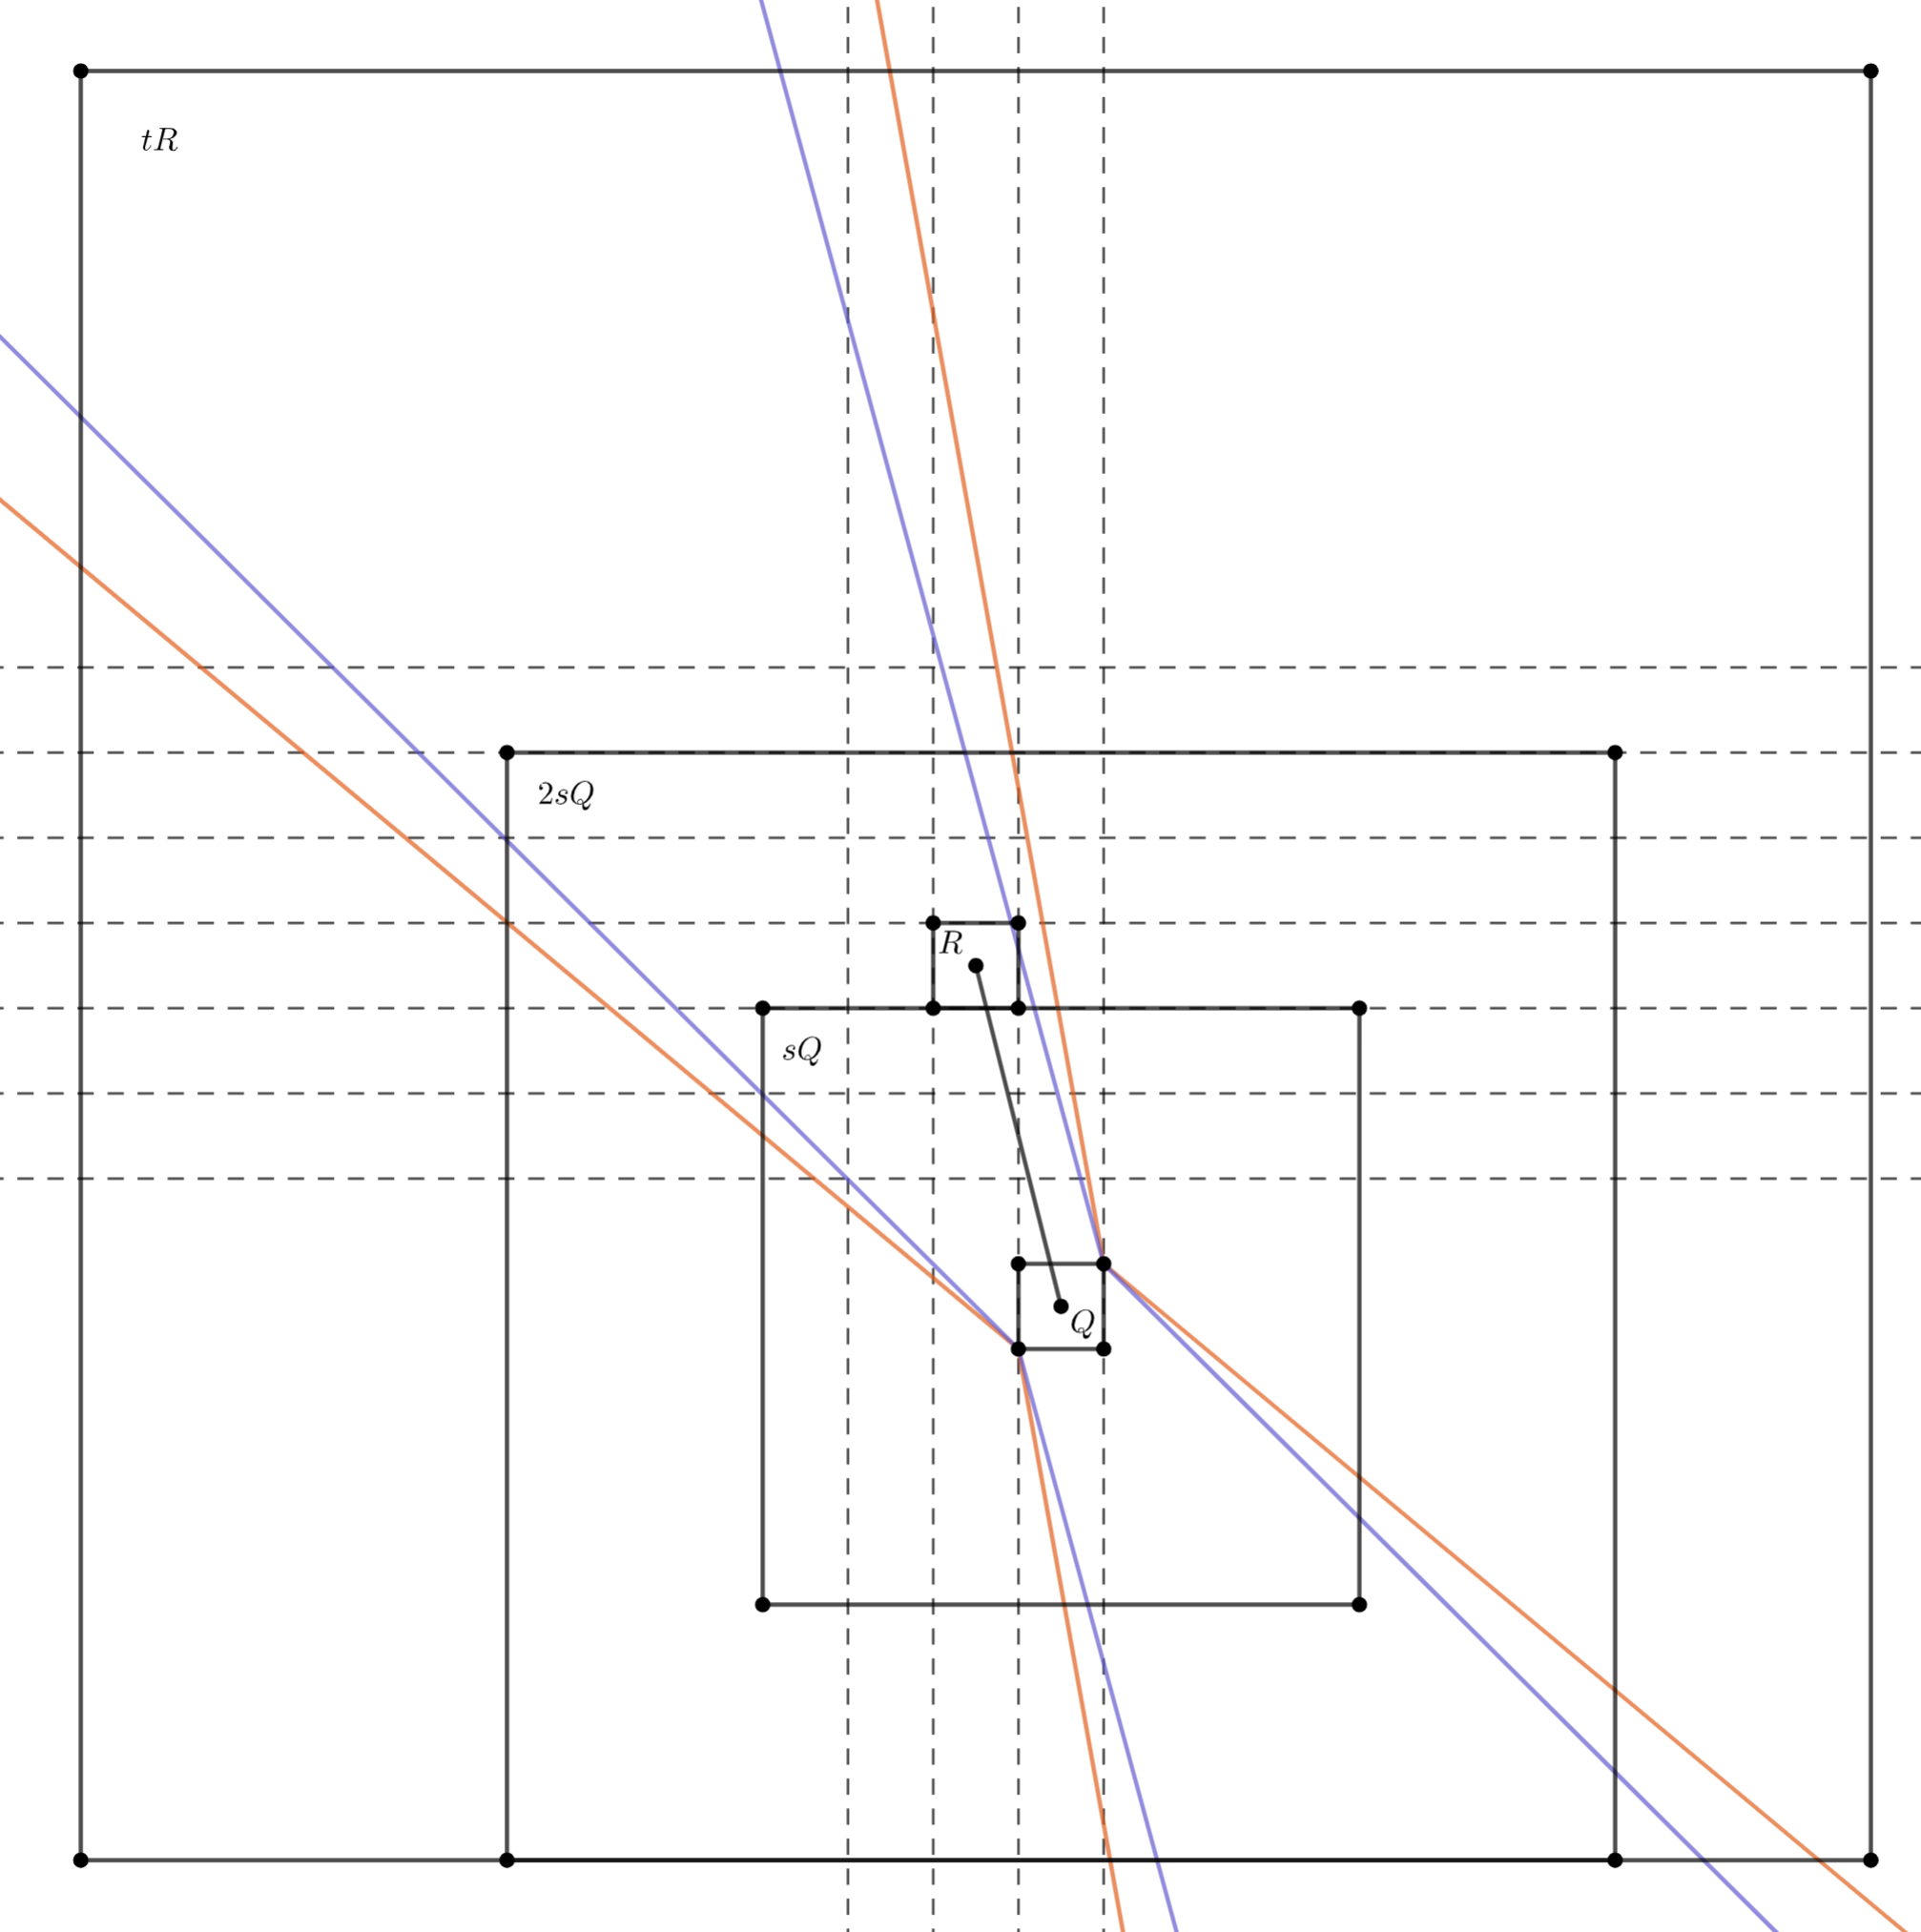
\includegraphics[width=.8\textwidth]{images/tRcover2sQ.png}
    \caption{An example in the proof on $\rr^2$}
\end{figure}


\newpage
\subsection{June 25-27 Modified Lemmas and New Lemmas}
\begin{lemma}
    If for $\mu$-a.e. $x\in \rr^2, \mu(B(x, 2r))\leq K\mu(B(x,r)), K\in\rr^+$, then
    $$\mu(5Q)\leq K^4 \mu(3Q)$$ where $Q$ is the dyadic cube, and $5Q$, $3Q$ are dilation cubes such that $\side 3Q = 3\side Q$, $\side 5Q = 5\side Q$, and $\centerof 5Q = \centerof 3Q = \centerof Q$.
\end{lemma}
\begin{proof} By the half open definition of the dyatic cube, for $\mu$-a.e. $x\in \rr^2$, $x$ must in only one cube $Q$. Let $r = \side Q /2$(in $\rr^2$). We first claim that $5Q\subset B(x, 16r)$ and $B(x, r)\subset 3Q$. As for any $q\in 5Q$, $|\centerof Q -x|\leq \sqrt{2}\cdot\side Q /2$ and $|\centerof 5Q -q|\leq \sqrt{2}\cdot\side 5Q /2 = 5\sqrt{2}\cdot \side Q/2$, 
    \begin{equation*}
        |x-q| = |x-\centerof Q + \centerof 5Q-q | \leq 3\sqrt{2}\cdot \side Q < \frac{16\side Q}{2} = 16r
    \end{equation*}
Then $q\in B(x, 16r)$ and thus $5Q\subset B(x, 16r)$. Similarly, for any $q^\prime\in B(x, r)$, 
\begin{equation*}
    |\centerof 3Q - q^\prime| = |\centerof Q - x + x-q^\prime| \leq \frac{\sqrt{2}\cdot\side Q}{2} + r < \frac{3\side Q}{2} = \frac{1}{2}\side 3Q
\end{equation*}
Then $q^\prime\in 3Q$ and thus $B(x, r)\subset 3Q$. Therefore, by the containments and the doubling measure condition, 
    \begin{equation}
        \mu(5Q) \leq \mu(B(x, 16r)) \leq K^4\mu(B(x,r))\leq K^4\mu(3Q)
    \end{equation}
\end{proof}

\begin{figure}[H]
    \centering
    \includegraphics[width=.56\textwidth]{images/doubleMucube.png}
    \caption{An example of containment in the proof on $\rr^2$}
\end{figure}


\begin{lemma}\label{lemma:CBQ2=0-carried}
    Let $\mu$ be a Radon measure on $\rr^n$, $V$ be an $m$-dimensional linear plane in $\rr^n$, $\alpha\in(0,1)$. Suppose $E\subset \rr^n$ such that for $\mu$-a.e. $x\in E$, and for every dyadic cube $Q$ containing $y$, 
    \begin{equation}\label{eq:muB2Q=0}
        \mu(C_\calB^2(Q, V, \alpha)) = 0
    \end{equation}
    Then $\mu$ is carried by $m$-Lipschitz graphs(i.e. $E$ is contained $\mu$-a.e. in an m-Lipschitz graph.)
\end{lemma}

\begin{proof}
    we first claim that if every dyadic cube $Q_k\ni x$ in the form of (\ref{eq:dyadiccube}) with side length $2^{-|k|}$ satisfies (\ref{eq:muB2Q=0}), 
    then
    \begin{equation}\label{eq:CBx=0}
        \mu(C_\calB(x, V, \alpha)) = 0
    \end{equation}
    Fix arbitrary $q_1\in Q_k$, if arbitrary $p\in C_\calB(q_1, V, \alpha)$, we have $\dist(p-q_1, V) > \alpha|p-q_1|$ by definition of bad cones. Now choose $\epsilon_p>0$ that satisfies $\dist(p-q_1, V) \geq \alpha (|p-q_1|+\epsilon_p)$. Then, for another point $q_2$ in $Q_k\ni q_1$, we have $|q_1-q_2|\leq \sqrt{n}\cdot 2^{-|k|}$. Hence, there exists a large enough $|k_p|$ such that $|q_1-q_2|<\alpha\epsilon_p/2<\epsilon_p/2$. Then,
    \begin{equation*}
        \begin{aligned} 
            \dist\left(p-q_2, V\right) & \geq \dist(p-q_1, V)-\left|q_1-q_2\right| \\ 
            & \geq \alpha(|p-q_1|+\epsilon_p)-\alpha(\epsilon_p / 2) \\ 
            & =\alpha(|p-q_1|+\epsilon_p / 2) \\ 
            & >\alpha\left(|p-q_1|+\left|q_2-q_1\right|\right) \\ 
            & \geq \alpha\left(\left|p-q_2\right|\right) 
    \end{aligned}
    \end{equation*}
    It follows that $p\in C_{\calB}^2(q_2, V, \alpha)$ and thus $p\in \bigcap_{q_i\in Q}C_\calB(q_i, V, \alpha) = C_\calB^2(Q_{k_p}, V, \alpha)$. Accordingly, for any $x\in E$, if any $p\in C_\calB(x, V, \alpha)$, then $p\in C_\calB(Q_k, V, \alpha)$, $x\in Q_k$ for some $|k|$, which implies
    \begin{equation}\label{eq:CBx-subset-UCBQ}
        p\in \bigcup_{|k|=1}^\infty C_\calB^2(Q_k, V, \alpha)\Rightarrow C_\calB(x, V, \alpha)\subset \bigcup_{|k|=1}^\infty \left\{C_\calB^2(Q_k, V, \alpha): Q_k\ni x\right\}
    \end{equation}
    Combining (\ref{eq:muB2Q=0}) and (\ref{eq:CBx-subset-UCBQ}), for $\mu$-a.e. $x\in E$,
    \begin{equation*}
        \mu(C_\calB(x, V, \alpha)) \leq \mu\left(\bigcup_{k=1}^\infty  \left\{C_\calB^2(Q_k, V, \alpha): Q_k\ni x \right \}\right) = 0
    \end{equation*}
    Therefore, (\ref{eq:CBx=0}) holds immediately and after applying corollary \ref{LisaCoro7.1}, we obtain the desired result.
\end{proof}

\newpage
\subsection{June 23-24 Lemma of Guarantee Distance Between Cubes}

\begin{lemma}\label{lemma:Guarantee-Distance-containQ-Between-2alpha}
    For $\alpha_1, \alpha_2\in(0,1), \alpha_1>\alpha_2$, a $m$-plane $V$ in $\rr^n$, a cube $Q$ with side length $2^{-|k|}$, and a cube $R$ with the same side length as $Q$, the distance bewteen the center of $R$ and the center of $Q$ has to satisfy
    \begin{equation*}
        |\centerof Q-\centerof R|\geq \left|\frac{2\sqrt{n} - 2\alpha_2}{\alpha_1-\alpha_2}-\sqrt{n}\right|\cdot 2^{-|k|}
    \end{equation*}
    to guarantee
    \begin{equation}\label{eq:condition-GDBC}
        R\in C_\calB^{1,1}(Q, V, \alpha_1) \quad\text{and}\quad R\in  C_\calB^{1,2}(Q, V, \alpha_2)
    \end{equation}
\end{lemma}
\begin{proof} 
    By assumption, there are some $x\in R\cap C_\calB^{1, 1}$ such that there exists $q\in Q$ and $x\in C_\calB(q, V, \alpha_1)$. Then $\dist(x-q, V) > \alpha_1|x-q|$. Now assume that $|x-q| = s\cdot 2^{-|k|}$. Then to satisfy (\ref{eq:condition-GDBC}), for any $y\in R$, there exists $q^\prime\in Q$ such that $y\in C_\calB(q^\prime, V, \alpha)$. Now we have $|x-y|\leq \sqrt{n}2^{-|k|}$, $|q-q^\prime|\leq \sqrt{n}2^{-|k|}$. Since $ |x-y| \geq|\dist (y-q^\prime, V)-\dist(x-q, V)| - |q-q^\prime|$, no matter $\dist (y-q^\prime, V)\lesseqgtr\dist(x-q, V)$,
    \begin{equation*}
        \begin{split}
            \dist(y-q^\prime, V) &\geq \dist(x-q, V)-|q-q^\prime|-|x-y| \\
            &> \alpha_1|x-q| - \sqrt{n}2^{-|k|+1}\\
            &= \alpha_1 s 2^{-|k|} - \sqrt{n}2^{-|k|+1}
        \end{split}
    \end{equation*}
    To guarantee that $\dist(y-q^\prime, V) > \alpha_2|y-q^\prime|$, we let $\alpha_1 s 2^{-|k|} - \sqrt{n}2^{-|k|+1} \geq  \alpha_2|y-q^\prime|$ then the assumption holds. Equivalently,
    \begin{equation*}
        \begin{split}
            \alpha_1 s 2^{-|k|} - \sqrt{n}2^{-|k|+1} &\geq  \alpha_2|y-q^\prime| \\
            &= \alpha_2 |x-q+y-x+q-q^\prime| \\
            &\geq \alpha_2||x-q|-|y-x|-|q-q^\prime||\\
            &\geq \alpha_2|s2^{-|k|}-2^{-|k|+1}|
        \end{split}
    \end{equation*}
    And we have 
    $$s\geq \frac{2\sqrt{n} - 2\alpha_2}{\alpha_1-\alpha_2}$$
    As $|q-\centerof Q|\leq \sqrt{n}2^{-|k|-1}$ and $|x-\centerof R| \leq \sqrt{n}2^{-|k|-1}$,
    \begin{equation*}
        \begin{split}
            |\centerof Q-\centerof R| &\geq ||x-q|-|x-\centerof R|-|q-\centerof Q|| \\
            &\geq\left|\frac{2\sqrt{n} - 2\alpha_2}{\alpha_1-\alpha_2}-\sqrt{n}\right|\cdot 2^{-|k|}
        \end{split}
    \end{equation*}
\end{proof}
\begin{figure}[H]
    \centering
    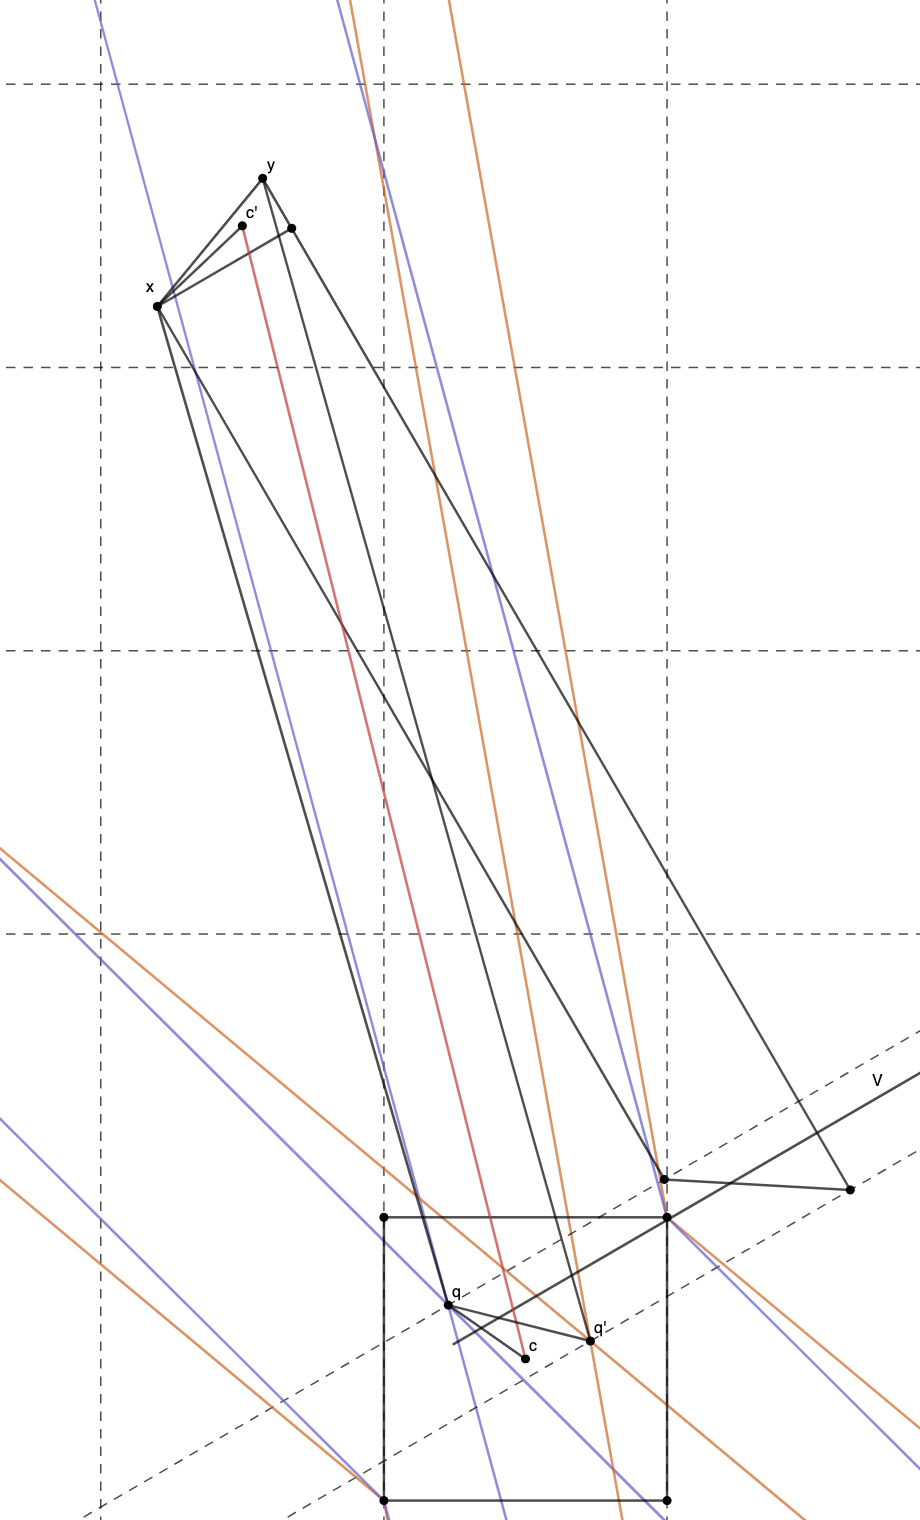
\includegraphics[width=.66\textwidth]{images/guaranteeContainalpha12.png}
    \caption{An example of containment in the proof on $\rr^2$}
\end{figure}




\newpage
\subsection{June 22 Doubling Measure for Cubes and other Lemmas}

\begin{lemma}\label{lemma:ofthmA} 
    Let $\mu$ be a pointwise doubling measure on $\rr^n$. For $\mu$-a.e. $x \in \rr^n$, $Q$ with side length $2^{-|k|}$ containing $x$, there is an $m$-plane $V$ and an $\alpha \in(0,1)$ such that with a scaling constant $s$,
    \begin{equation}\label{eq:lemmaofthmAeq}
        \lim_{|k| \rightarrow \infty} \frac{\mu\left(C_\calB(Q, V, \alpha)\right)}{\mu(sQ))}=0
    \end{equation}
    if and only if $\mu$ is carried by Lipschitz graphs.
\end{lemma}
\textit{Proof for Sufficient Condition.} With the same notation in Lemma \ref{lemma:CBQ2carried}, where $E = \bigcup_{i=1}^\infty E_i$ and for $\mu$-a.e. $y\in E$, $E_i = Q_{E_i}\cap E$. Fix a $Q_{E_i}$, by (\ref{eq:lemmaofthmAeq}), for any $\epsilon>0$, there exists $N_i\in\nn$ such that when $k\geq N_i$, 
$$\left |\frac{\mu\left(C_\calB^2(Q_{E_i}, V, \alpha)\right)}{\mu(sQ_{E_i}))}\right | < \epsilon$$
Define $r = 2^{-|k|}s$, then $\lim_{|k|\rightarrow\infty} r = 0$. Thus, there exists $N^\prime\in \nn$ such that whenever $k\geq N^\prime$, $|r|<\epsilon$. Thus, choosing $N=\max\{\{N_i\}\cup\{N^\prime\}$, two inequalities hold for every $Q_{E_i}$ in the meanwhile. Then for $\mu$-a.e. $y\in Q_{E_i}$ and by (\ref{eq:CysubsetCQ}), $s\cdot Q_{E_i}\subset B(y, r)$ and $C_\calB(y, r, V, \alpha)\subset C_\calB(y, V, \alpha)\subset C_\calB^2(Q_{E_i}, V, \alpha)$. Thus, let $\delta = \epsilon$, we have for any $\epsilon>0$ there exists $\delta>0$ such that whenever $|r-0|<\delta$, by containment, 
\begin{equation}
    \left|  \frac{\mu(C_\calB(y, r, V, \alpha))}{\mu(B(y, r))} \right| \leq \left |\frac{\mu\left(C_\calB^2(Q_{E_i}, V, \alpha)\right)}{\mu(sQ_{E_i}))}\right| < \epsilon
\end{equation}
Therefore
\begin{equation}\label{eq:lemmathmAeq2}
    \lim_{r\downarrow 0} \frac{\mu(C_\calB(y, r, V, \alpha))}{\mu(B(y, r))} = 0
\end{equation}
Applying \ref{thm:NaplesthmD}, the conclusion holds.


\begin{customthm}{{\cite[Theorem D]{naples2020}}}\label{thm:NaplesthmD}
    Let $\mu$ be a pointwise doubling measure on a separable, finite or infinite dimensional Hilbert space $H$. For $\mu$-a.e. $x \in H$ there is an $m$ -plane $V$ and an $\alpha \in(0,1)$ such that
$$
\lim _{r \downarrow 0} \frac{\mu\left(C_{\mathcal{B}}(x, r, V, \alpha)\right)}{\mu(B(x, r))}=0
$$
if and only if $\mu$ is carried by Lipschitz graphs.
\end{customthm}




\begin{lemma}
    If $\mu$-a.e. $x\in \rr^n, \mu(B(x, 2r))\leq K\mu(B(x,r)), K\in\zz^+$, then
    $\mu(2Q)\leq K^3 \mu(Q)$ where $Q$ is the dyadic cube, 2$Q$ is the cube with double dilation of $Q$. 
\end{lemma}
\begin{proof} By the half open definition of the dyatic cube, for $\mu$-a.e. $x\in \rr^n$, $x$ must in only one cube, named $Q$ with $\side Q = 2^{-|k|}$. Let $r = \frac{1}{2}\side Q$, then by the containment
    \begin{equation}
        \mu(4Q)\leq \mu(B(x, 8r))\leq K^3 \mu(B(x, r)) \leq K^3 \mu(2Q)
    \end{equation}

    \begin{equation}
        \mu(5Q) \leq \mu(B(x, 16r)) \leq K^4\mu(B(x,r))\leq K^4\mu(3Q)
    \end{equation}
\end{proof}
There always exists $k$ such that any $\mu$-a.e. $x$ must in $1/2 Q$ with side length $2^{-|k|}$. Then similarly we have $\mu(2Q)\leq K^3\mu(Q)$.

\begin{figure}[H]
    \centering
    \includegraphics[width=.66\textwidth]{images/doubleMucube.png}
    \caption{An example of containment in the proof on $\rr^2$}
\end{figure}

\newpage
\subsection{June 21 \texorpdfstring{$\lim_{Q\rightarrow x}\mu(C_\calB(Q, V, \alpha))/\mu(sQ) = 0$}{Lg}}

\begin{definition}[Alternative Definition for Bad Cones at a Cube] For the dyadic cube $Q$, let $R$ denote the dyadic cube with the same side length as $Q$ in the cube system. Then definitions of bad cones at a cube can be 
    \begin{equation*}
        C_\calB^{k,1}(Q, V, \alpha) = \{R: R\cap C_\calB^k(Q, V, \alpha) \neq \emptyset\}, \quad
        C_\calB^{k,2}(Q, V, \alpha) = \{R: R\subset C_\calB^k(Q, V, \alpha)\} 
    \end{equation*}
for $k=1,2$.
\end{definition}




\begin{customthm}{A}\label{thmA} 
    Let $\mu$ be a pointwise doubling measure on $\rr^n$. For $\mu$-a.e. $x \in \rr^n$, $Q$ that contains $x$, there is an $m$-plane $V$ and an $\alpha \in(0,1)$ such that with a scaling constant $s$,
    \begin{equation}\label{thmAeq}
        \lim_{Q \downarrow x} \frac{\mu\left(C_\calB(Q, V, \alpha)\right)}{\mu(sQ))}=0
    \end{equation}
    if and only if $\mu$ is carried by Lipschitz graphs.
\end{customthm}
\textit{Proof for Sufficient Condition.} With the same notation in Lemma \ref{lemma:CBQ2carried}, where $E = \bigcup_{i=1}^\infty E_i$ and for some $y_i\in E$, $E_i=\{y_i\}\subset Q_{E_i}$. Fix $y_0\in Q_{E_i}$ and by (\ref{eq:CysubsetCQ}), when $|k|\downarrow 0$, $C_\calB(y_0, V, \alpha)\subset C_\calB^2(Q_{E_i}, V, \alpha)$. Then if $r=s\cdot 2^{-|k|}$, we have $s\cdot Q_{E_i}\subset B(y_0, r)$ and $C_\calB(y_0, r, V, \alpha)\subset C_\calB(y_0, V, \alpha)\subset C_\calB^2(Q_{E_i}, V, \alpha)$. Now as $|k|\downarrow 0\Rightarrow r\downarrow 0$ and by (\ref{thmAeq}),
\begin{equation}\label{eq:thmAeq1}
    \lim_{r\downarrow 0} \frac{\mu(C_\calB(y_i, r, V, \alpha))}{\mu(B(y_i, r))} \leq \lim_{Q \downarrow x} \frac{\mu\left(C_\calB(Q, V, \alpha)\right)}{\mu(sQ))}=0
\end{equation} 
Applying \ref{eq:thmAeq1} for every $y$ in every $Q_{E_i}$, and \ref{thm:NaplesthmD}, the conclusion holds.




\newpage
\subsection{June 17-20 \texorpdfstring{$\mu(C_\mathcal{B}^2(Q, V, \alpha)) = 0 \Rightarrow \mu$ Carried by Lipschitz Graph}{Lg}}

\begin{lemma}\label{lemma:CBQ2carried}
    Let $\mu$ be a Radon measure on $\rr^n$, $V$ be an $m$-dimensional linear plane in $\rr^n$, $\alpha\in(0,1)$. Suppose $E\subset \rr^n$ such that for $\mu$-a.e. $y\in E$, and for every dyadic cube $Q$ containing $y$, 
    \begin{equation}\label{muB2=0}
        \mu(C_\calB^2(Q, V, \alpha)) = 0
    \end{equation}
    Then $\mu$ is carried by $m$-Lipschitz graphs(i.e. $E$ is contained $\mu$-a.e. in an m-Lipschitz graph.)
\end{lemma}

\begin{proof}
    we first claim that if every dyadic cube $Q\ni y$ in the form of (\ref{eq:dyadiccube}) with side length $2^{-|k|}$ satisfies (\ref{muB2=0}), 
    then
    \begin{equation}\label{muBx=0}
        \mu(C_\calB(y, V, \alpha)) = 0
    \end{equation}
    Note that each $y\in E$ is contained in no more than one half open $Q$. Let $Q_{E_i}$ denote the dyadic cube that contains $E_i\subset E$ such that $E_i$ consists of all $y\in E\cap Q_{E_i}$ and $E$ is the countable union of disjoint $E_i$. For any two points $x_1\in Q_{E_i}, y_1\in E_i$, we have $|x_1-y_1|\leq \sqrt{n}\cdot 2^{-|k|}$. Consider that if any $p\in C_\calB(y_1, V, \alpha)$, we have $\dist(p-y_1, V) > \alpha|p-y_1|$ by definition of bad cones. Now let $\epsilon>0$ such that $\dist(p-y_1, V) \geq \alpha (|p-y_1|+\epsilon)$. When $|k|\rightarrow \infty, 2^{-|k|}\rightarrow 0$, so there exists $N\in\nn$ such that whenever $|k|\geq N$, for $x_1, y_1\in Q_{E_i}$ we have $|x_1-y_1|<\alpha\epsilon/2<\epsilon/2$, recalling that $\alpha\in(0,1)$. Then
\begin{equation*}
    \begin{aligned} 
        \dist\left(p-x_1, V\right) & \geq \dist(p-y_1, V)-\left|x_1-y_1\right| \\ 
        & \geq \alpha(|p-y_1|+\epsilon)-\alpha(\epsilon / 2) \\ 
        & =\alpha(|p-y_1|+\epsilon / 2) \\ 
        & >\alpha\left(|p-y_1|+\left|x_1-y_1\right|\right) \\ 
        & \geq \alpha\left(\left|p-x_1\right|\right) 
\end{aligned}
\end{equation*}
It follows that $p\in C_{\calB}(x_1, V, \alpha)$, and as $x_1$ is arbitrary point in $Q_{E_i}$, $p\in C_\calB^2(Q_{E_i}, V, \alpha)$. Thus, when $|k|\rightarrow \infty$
\begin{equation}\label{eq:CysubsetCQ}
    C_{\calB}(y_1, V, \alpha)\subset C_\calB(Q_{E_i}, V, \alpha),\quad \forall y_1\in E_i \subset Q_{E_i}
\end{equation}
Then applying (\ref{muB2=0}), 
\begin{equation*}
    \begin{split}
        \mu(\bigcup_{y\in E}C_\calB(y, V, \alpha))
        = \lim_{|k|\rightarrow \infty}\mu\left( \bigcup_{E_i\in E}\bigcup_{y\in Q_{E_i}} C_\calB(y, V, \alpha) \right)  
        \leq \lim_{|k|\rightarrow\infty}\mu\left( \bigcup_{E_i\in E} C_\calB^2(Q_{E_i}, V, \alpha) \right)
        = 0
    \end{split}
\end{equation*}
Therefore, we have (\ref{muBx=0}) for each $y\in E$. Then applying corollary \ref{LisaCoro7.1}, we obtain the desired result. 
\end{proof}



An example of this proof illustrated in $\rr^2$ is shwon in Figure \ref{fig:CB1=CB2}.

\begin{figure}[H]
    \centering
    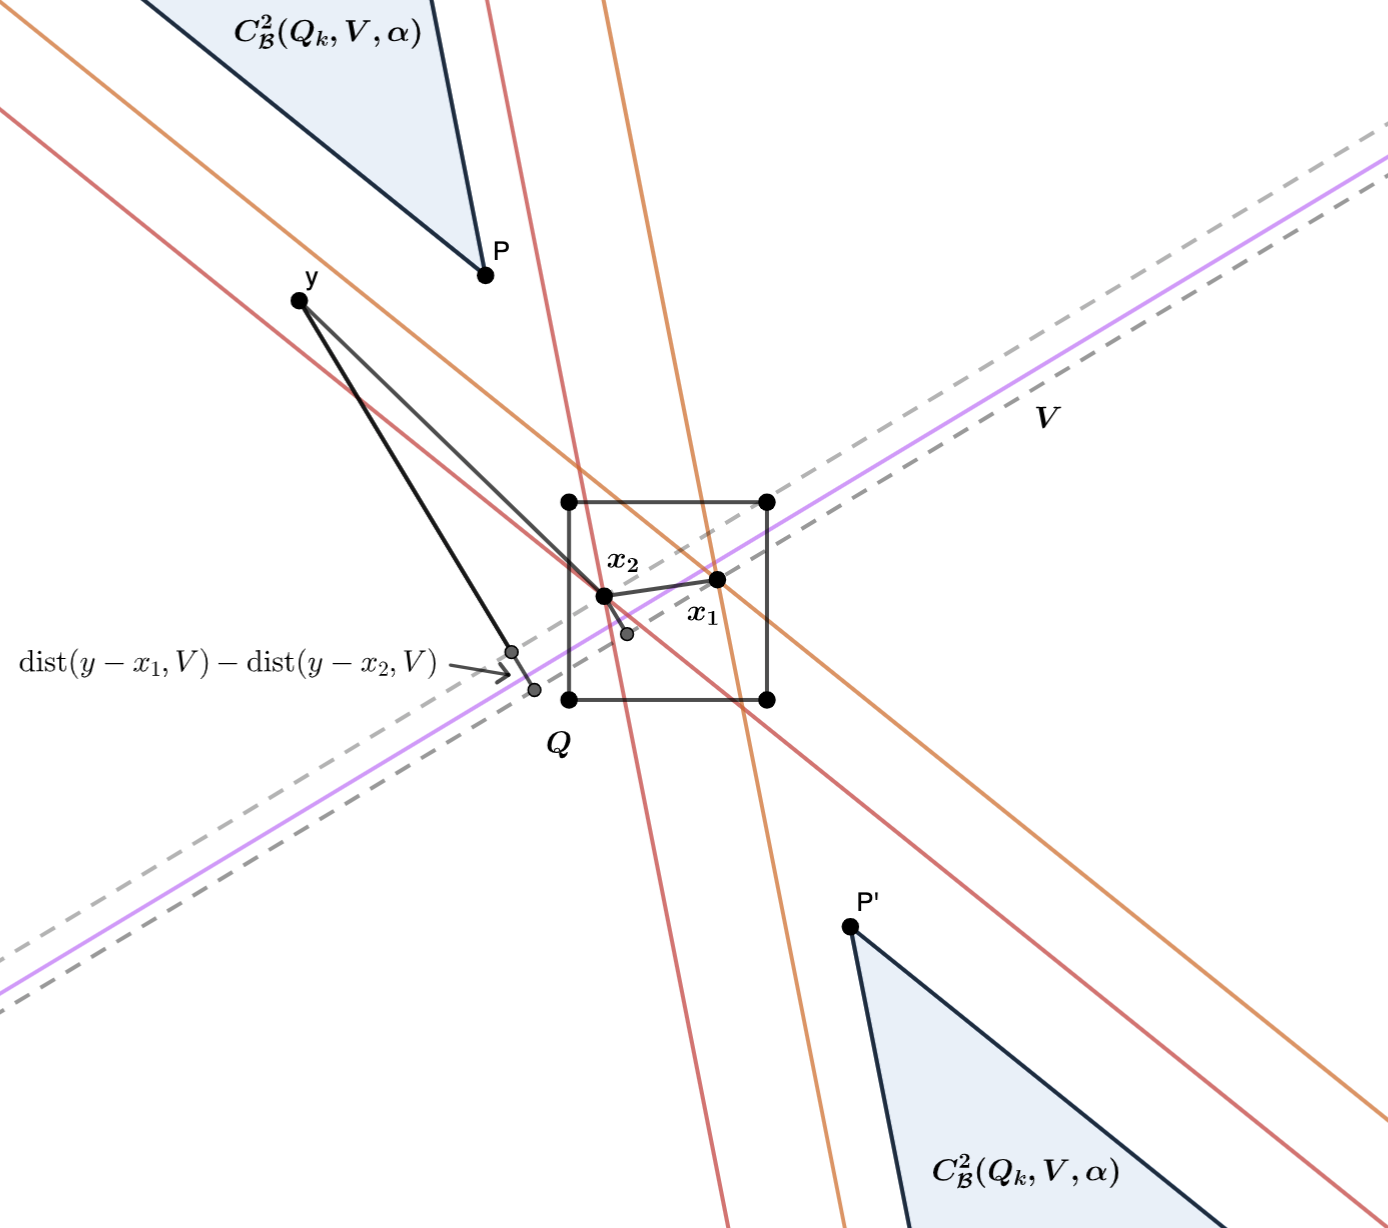
\includegraphics[width=.6\textwidth]{images/CB1=CB2.png}
    \caption{Example visulization of proof in $\rr^2$}
    \label{fig:CB1=CB2}
\end{figure}


\begin{corollary}[{\cite[Corollary 7.1]{naples2020}}]
    Let $\mu$ be a Radon measure on $H, V$ be an $m$-dimensional linear plane in $H$, $\alpha \in(0,1)$, and $0<r<\infty$. If for $\mu$ -a.e. $x \in H$
   $$
   \mu\left(C_{\mathcal{B}}(x, r, V, \alpha)\right)=0
   $$
   then $\mu$ is carried by $m$-Lipschitz graphs.
\end{corollary}




\newpage
\subsection{June 16 New Cone Definition for Dyadic Cubes}
\begin{definition}[Dyadic Cubes] A dyadic cube $Q$ is a set of the form
    \begin{equation}\label{eq:dyadiccube}
        Q=\left[\frac{j_{1}}{2^{k}}, \frac{j_{1}+1}{2^{k}}\right) \times \cdots \times\left[\frac{j_{n}}{2^{k}}, \frac{j_{n}+1}{2^{k}}\right), \quad k, j_{1}, \ldots, j_{n} \in \mathbb{Z}
    \end{equation}
\end{definition}

\begin{definition}[Bad Cone at a Cube(definition 1)] Let $Q$ be the dyadic cube, then we can have the first definition of bad cone at $Q$ with respect to $V$ and $\alpha$ by:
    $$C^1_{\mathcal{B}}(Q, V, \alpha) := \bigcup_{x\in Q} C_\mathcal{B}(x, V, \alpha), \quad C^1_{\mathcal{B}}(Q, r, V, \alpha) = C^1_{\mathcal{B}}(Q, V, \alpha) \cap B(x,r)$$
    where $V$ is a m-dimensional linear plane through the origin. 
\end{definition}

\begin{definition}[Bad Cone for Cube(definition 2)]
    We can have the second definition of bad cone at $Q$ with respect to $V$ and $\alpha$ with the similar notation:
    $$C^2_{\mathcal{B}}(Q, V, \alpha) := \bigcap_{x\in Q} C_\mathcal{B}(x, V, \alpha), \quad
    C^2_{\mathcal{B}}(Q, r, V, \alpha) = C^2_{\mathcal{B}}(Q, V, \alpha) \cap B(x,r)
    $$
\end{definition}
\begin{figure}[H]
    \centering
    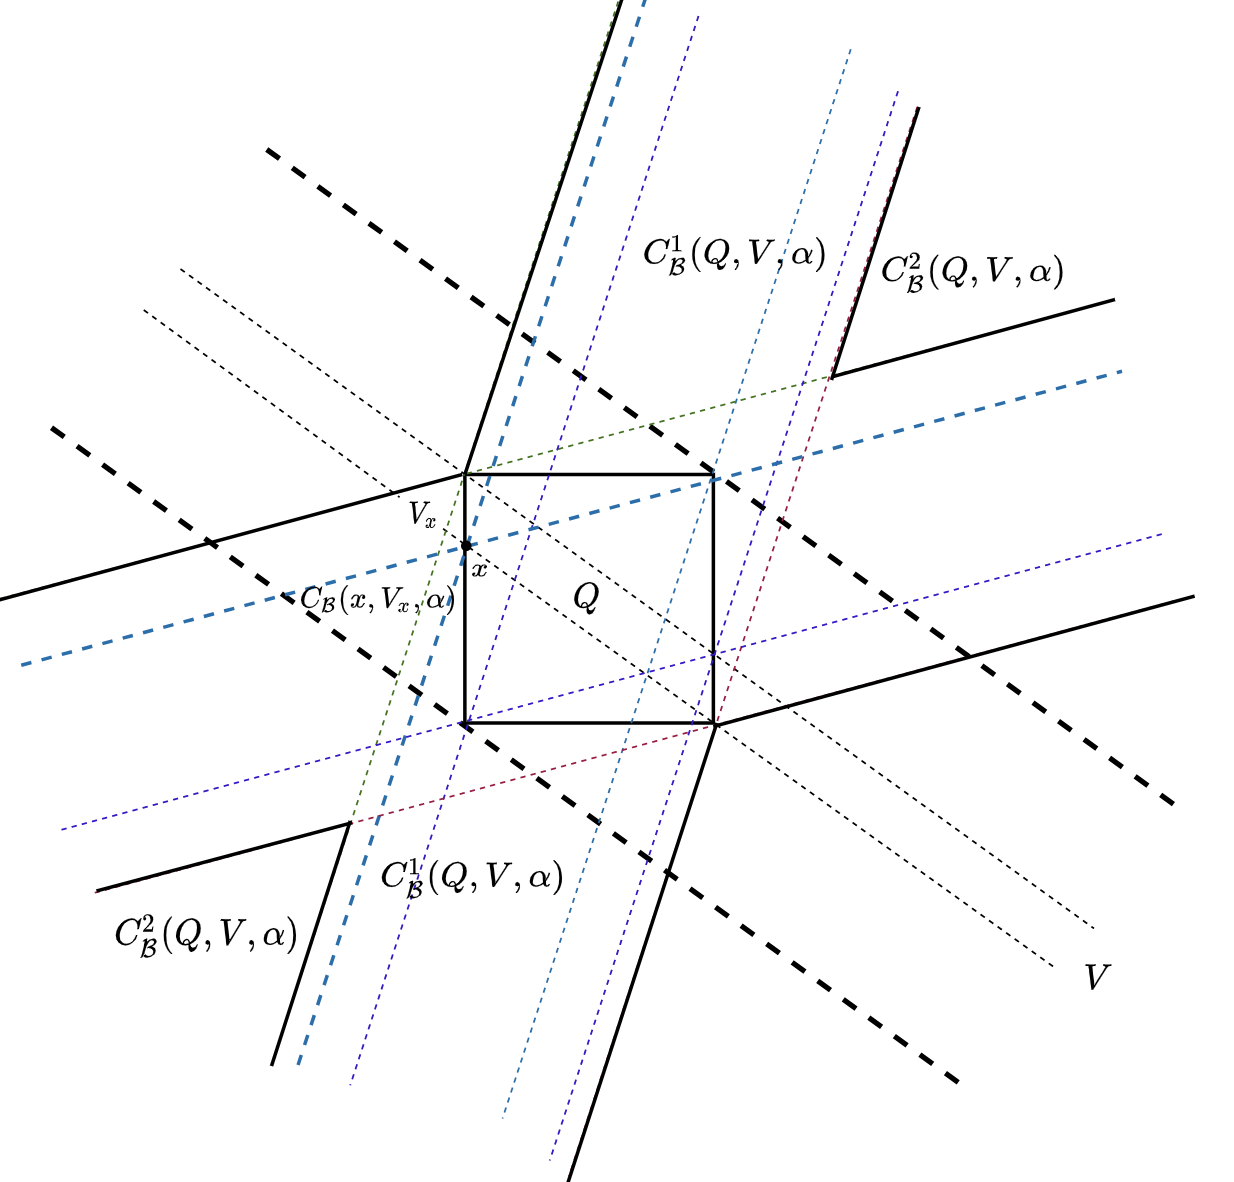
\includegraphics[width=.66\textwidth]{images/cubebadconeDef.png}
    \caption{Visulize two definitions of bad cone at a cube in $\rr^2$}
\end{figure}

\begin{problem}
    Suppose that at $\mu$-a.e. $x$, $\alpha\in(0, 1)$, for all $k$, for every cube $Q\ni x$ of side length $2^{-k}$ satisfies
    $$
    \mu(C^2_\mathcal{B}(Q, V, \alpha)) = 0
    $$ 
    is $\mu$-carried Lipschitz by Lipschitz graphs?
\end{problem}

\newpage
\subsection{June 15 A Proposition of Doubling Measure for Cubes}

\begin{proposition}
    If $\forall x\in \rr^2, \mu(B(x, 2r))\leq K\mu(B(x,r)), K\in\zz^+$, then $\exists R\in \zz^+$ s.t. $\mu(3Q)\leq R\mu(Q)$ where $Q$ is the cube, 3$Q$ is the cube with triple side length with same center as $Q$. 
\end{proposition}
\proof  $\mu(3Q) \leq \mu(B(x, 4\side Q)) \leq K^3\mu(B(x, \frac{1}{2} \side r))\leq K^3 \mu(Q)$ due to doubling measure and containment. 

\begin{figure}[H]
    \centering
    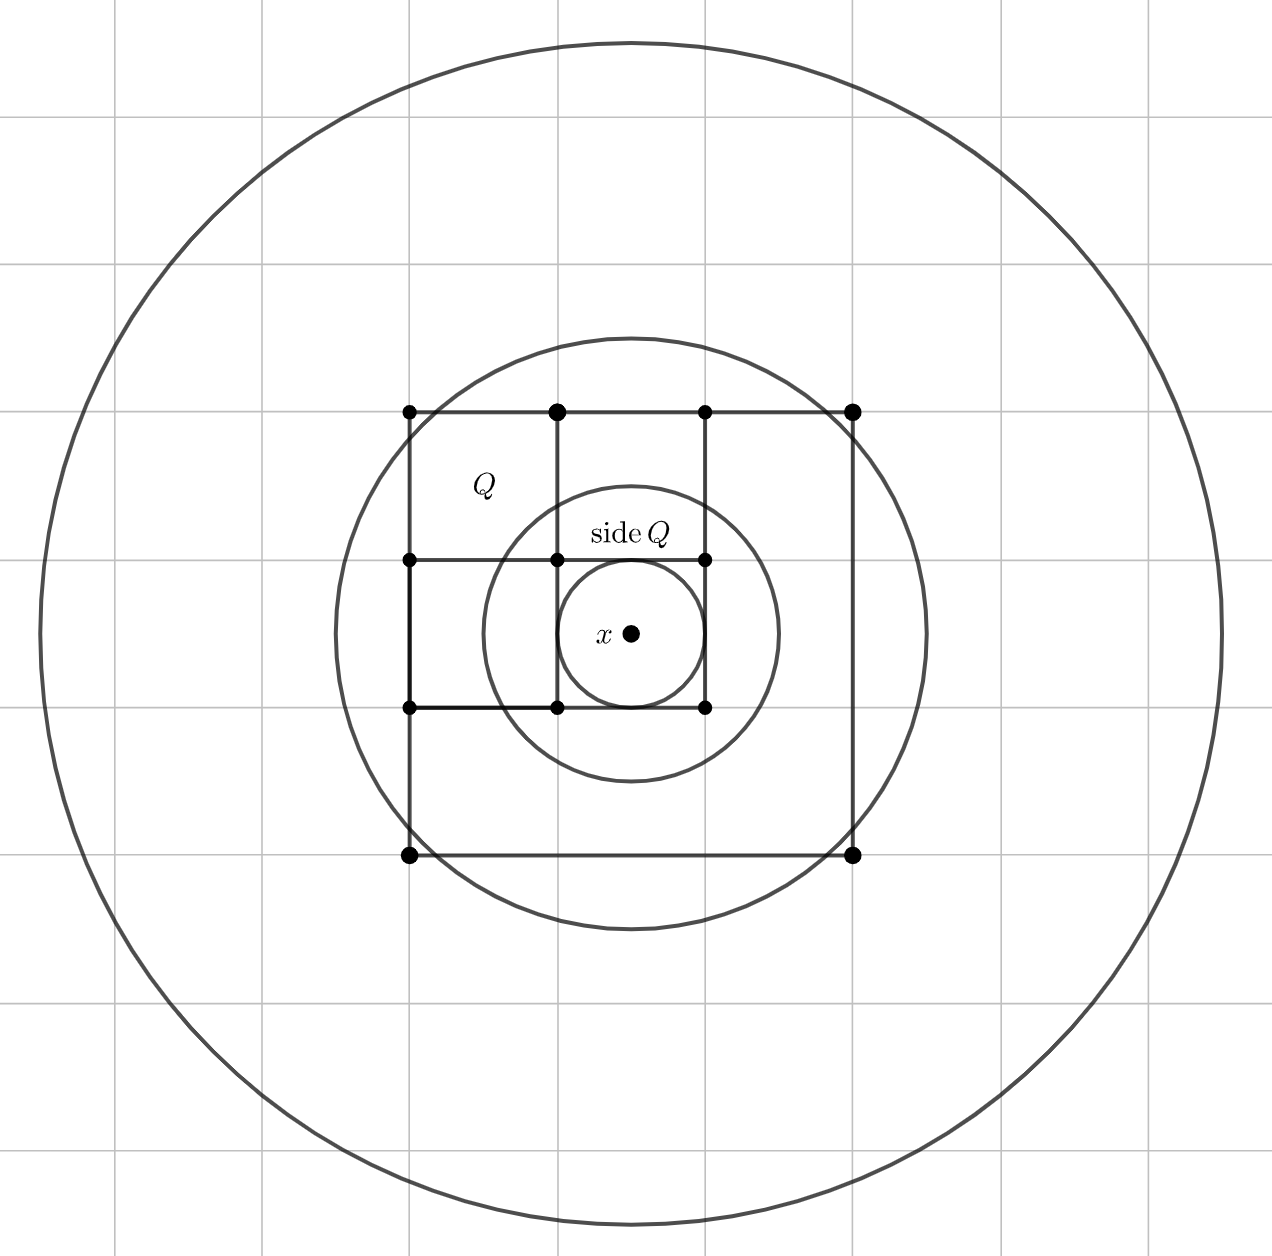
\includegraphics[width=.66\textwidth]{images/tripleMcube.png}
\end{figure}


\newpage
\subsection{June 14 Paper \texorpdfstring{\cite{naples2020}}{Lg} Sec. 7 Graph Rectifiable Measures}

\begin{definition}[Good Cone]
    Let $V$ be a m-dimensional plane in Hilbert space $H$, then we can define the good cone at $x$ with respect to $V$ and $\alpha$ by:
    $$
    C_\mathcal{G}(x, V, \alpha) := \{y\in H: \dist(y-x, V) \leq \alpha |x-y|\}
    $$
    another notation:
    $$
    C_\mathcal{G}(x, r, V, \alpha) = C_\mathcal{G}(x, V, \alpha) \cap B(x, r)
    $$
\end{definition}
\begin{definition}[Bad Cone]
    The bad cone at x with respect to V and $\alpha$:
    $$
    C_\mathcal{B}(x, V, \alpha) := H\setminus C_{\mathcal{G}(x, V, \alpha)}, \quad C_\mathcal{B}(x, r, V, \alpha) = C_\mathcal{B}(x, V, \alpha) \cap B(x, r)
    $$
\end{definition}


\begin{figure}[H]
    \centering
    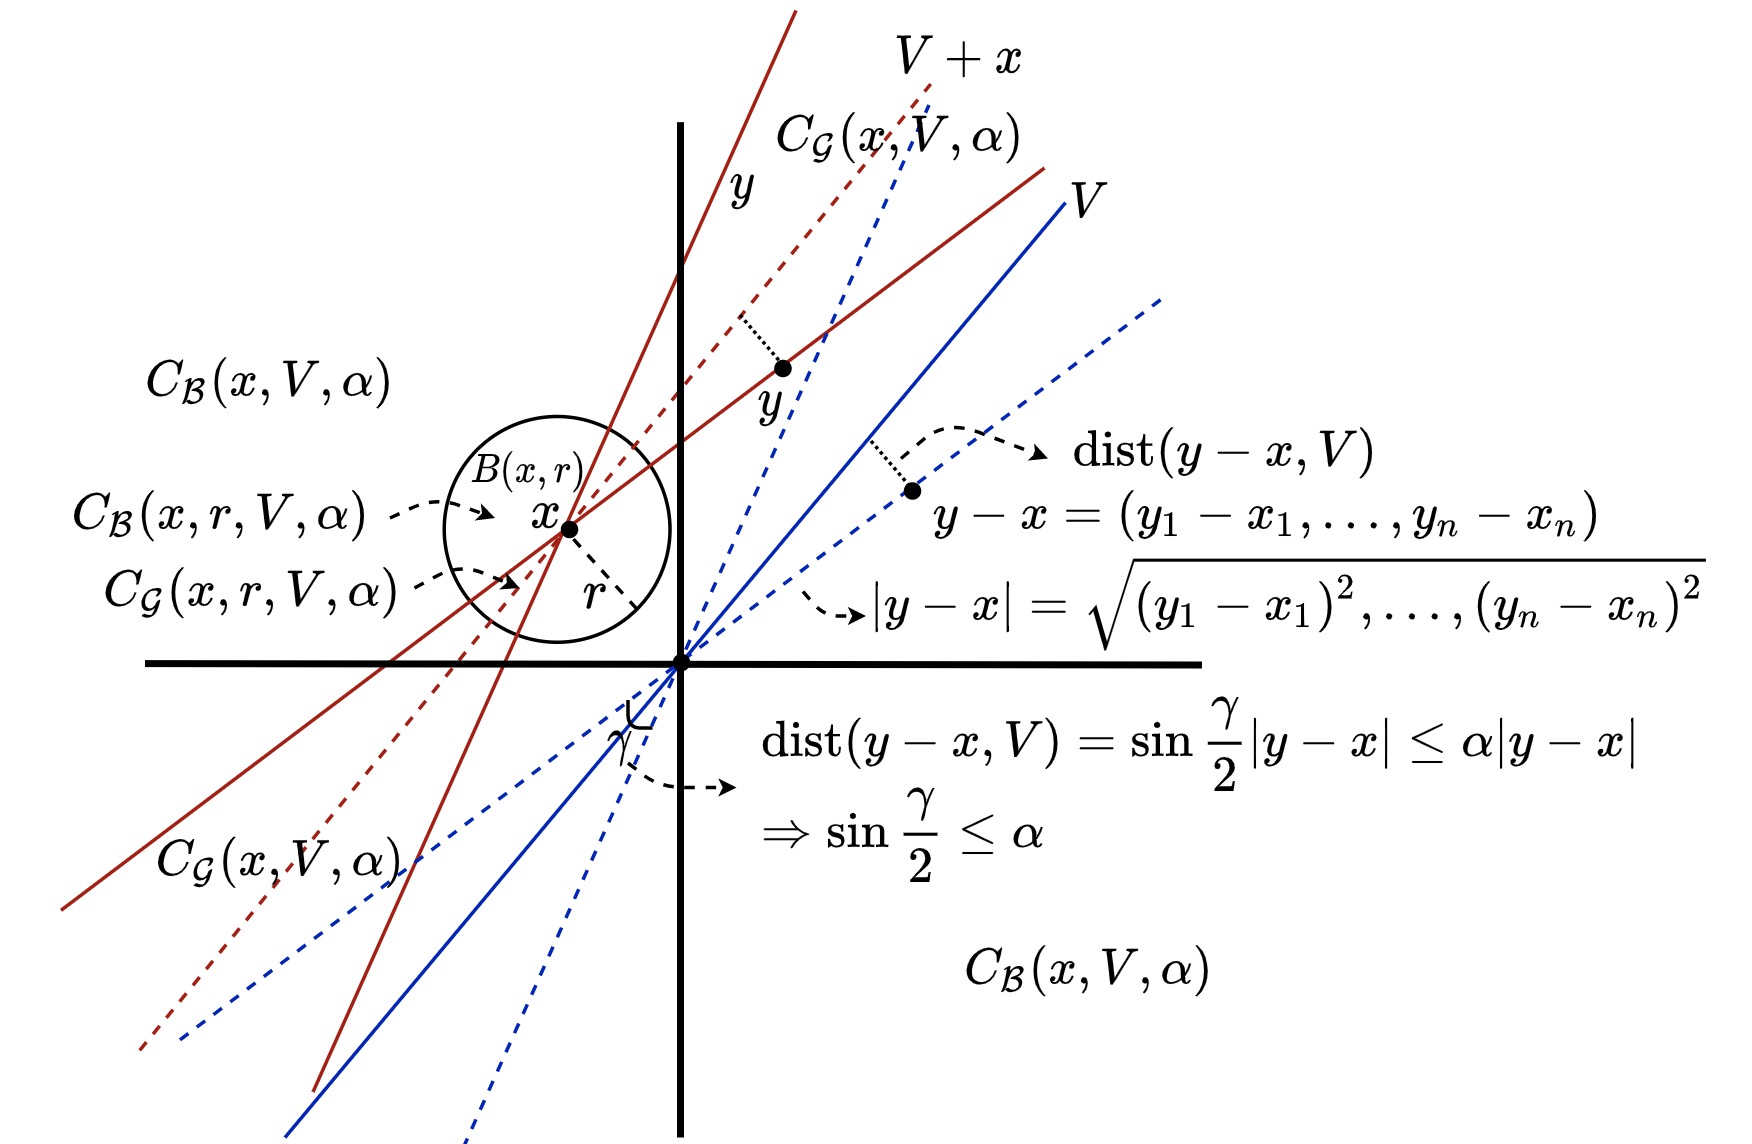
\includegraphics[width=.8\textwidth]{images/conedef.png}
    \caption{Example visualization of definitions related to cones in $\rr^2$}
\end{figure}

\begin{definition}[Carried $\&$ Singular]
   Let $(\mathbb{X}, \mathcal{M})$ be a measurable space, and let $\mathcal{N} \subset \mathcal{M}$ be a family of measurable sets. We say
   \begin{enumerate}[(1)]
       \item $\mu$ is carried by $\mathcal{N}$ if there exist countably many $N_{i} \in \mathcal{N}$ such that $\mu\left(\mathbb{X} \backslash \bigcup_{i} N_{i}\right)=0$;
       \item $\mu$ is singular to $\mathcal{N}$ if $\mu(N)=0$ for every $N \in \mathcal{N}$.    
   \end{enumerate}
   A $\sigma$ -finite measure $\mu$ on $(\mathbb{X}, \mathcal{M})$ can be decomposed uniquely as
       $$
       \mu=\mu_{\mathcal{N}}+\mu_{\mathcal{N}}^{\perp}
       $$
       where $\mu_{\mathcal{N}}$ is carried by $\mathcal{N}$ and $\mu_{\mathcal{N}}^{\perp}$ is singular to $\mathcal{N}$. 
\end{definition}

\begin{theorem}[Theorem 7.1 Geometric Lemma] $ $\\
    Let $F \subset H$, let $V$ be an $m$-dimensional linear plane in $H$, and let $\alpha \in(0,1) .$ If
$$
F \backslash C_{\mathcal{G}}(x, V, \alpha)=\emptyset \text { for all } x \in F
$$
then $F$ is contained in an $m$ -Lipschitz graphs. In particular, $F \subset \Gamma$ where $\Gamma$ is a Lipschitz graph with respect to $V$ and the Lipschitz constant corresponding to $\Gamma$ is at most $1+1 /\left(1-\alpha^{2}\right)^{1 / 2} .$
\end{theorem}
\proof Let $x \in F$. Let $P_{V}: H \rightarrow V$ denote standard projection onto the $m$ -plane $V$. Suppose that $\left|P_{V} x-P_{V} y\right|<\left(1-\alpha^{2}\right)^{1 / 2}|x-y|$. Then $y \in C_{\mathcal{B}}(x, V, \alpha)$, and by assumption of $F$ this means that $y \notin F$. Thus we may assume that if $x, y \in F$ then
$$
\left|P_{V} x-P_{V} y\right| \geq\left(1-\alpha^{2}\right)^{1 / 2}|x-y|
$$
From this inequality we see that $P_{V} \mid F$ is one-to-one with Lipschitz inverse $f=\left(P_{V} \mid F\right)^{-1}$ and $\operatorname{Lip}(f) \leq\left(1-\alpha^{2}\right)^{-1 / 2}$. Note that $F=f\left(P_{V} \mid F\right)$. Then there exists a Lipschitz extension $\tilde{f}: V \rightarrow$ $H$ so that $F \subset \tilde{f}(V)$. Thus the desired result holds. 

\begin{corollary}[Corollary 7.1]
 Let $\mu$ be a Radon measure on $H, V$ be an $m$-dimensional linear plane in $H$, $\alpha \in(0,1)$, and $0<r<\infty$. If for $\mu$ -a.e. $x \in H$
$$
\mu\left(C_{\mathcal{B}}(x, r, V, \alpha)\right)=0
$$
then $\mu$ is carried by $m$ -Lipschitz graphs.
\end{corollary}
\proof Let $F$ denote the set of $x \in H$ that satisfy (18). We may assume $F \subset B(0, r / 2)$; otherwise we may write $F$ as a union of countably many sufficiently small sets and show that each one is $m$ -graph rectifiable. Let $\left\{x_{i}\right\}$ be a countable dense subset of $F .$ It follows from (18) and the containment $F \subset B(0, r / 2)$ that for each $x_{i}$ there exists $F_{i} \subset F$ such that
$$
F_{i} \cap C_{\mathcal{B}}\left(x_{i}, r, V, \alpha\right)=F_{i} \cap C_{\mathcal{B}}\left(x_{i}, V, \alpha\right)=\emptyset
$$
and $\mu\left(F \backslash F_{i}\right)=0$. Define $F^{\prime}:=\bigcap_{i=1}^{\infty} F_{i}$. Then
$$
\mu\left(F \backslash F^{\prime}\right)=\mu\left(F \backslash \bigcap_{i=1}^{\infty} F_{i}\right)=\mu\left(\bigcup_{i=1}^{\infty} F \backslash F_{i}\right) \leq \sum_{i=1}^{\infty} \mu\left(F \backslash F_{i}\right)=0
$$
We claim that $F^{\prime} \cap C_{\mathcal{B}}(x, V, \alpha)=\emptyset$ for every $x \in F^{\prime} .$ Fix $x \in F^{\prime}$, and let $y \in C_{\mathcal{B}}(x, V, \alpha)$.
By definition of bad cone we have that $\dist(y-x, V)>\alpha|y-x|$. Now let $\epsilon>0$ such that $\dist(y-x, V) \geq \alpha(|y-x|+\epsilon)$. Recalling that $0<\alpha<1$, choose $x_{i}$ such that $\left|x_{i}-x\right|<\alpha \epsilon / 2<$
$\epsilon / 2 .$ Then
$$
\begin{aligned}
\dist\left(y-x_{i}, V\right) & \geq \dist(y-x, V)-\left|x-x_{i}\right| \\
& \geq \alpha(|y-x|+\epsilon)-\alpha(\epsilon / 2) \\
&=\alpha(|y-x|+\epsilon / 2) \\
&>\alpha\left(|y-x|+\left|x_{i}-x\right|\right) \\
& \geq \alpha\left(\left|y-x_{i}\right|\right) .
\end{aligned}
$$
In particular, we conclude that $y \in C_{\mathcal{B}}\left(x_{i}, V, \alpha\right) .$ Since $F_{i} \cap C_{\mathcal{B}}\left(x_{i}, V, \alpha\right)=\emptyset$, it must be that case that $y \notin F_{i}$. It follows that $y \notin F^{\prime}$, and thus $F^{\prime} \cap C_{\mathcal{B}}(x, V, \alpha)=\emptyset$ for all $x \in F^{\prime}$. By an application of Theorem $7.1$ we conclude that there exists an $m$ -Lipschitz graph $\Gamma$ such that $F^{\prime} \subset \Gamma$, so $\mu(F \backslash \Gamma)=0$.

\begin{lemma}[Lemma 7.2]
    Let $\mu$ be a Radon measure on $H$. For $x_{0} \in H, V$ an $m$-dimensional linear plane, $\alpha \in(0,1)$, and parameter $K>0$, let $E$ denote the set of points $x \in H$ such that
(i) The sequence of functions
$$
f_{r}(x):=\frac{\mu\left(C_{\mathcal{B}}(x, r, V, \alpha)\right)}{\mu(B(x, r))}
$$
converges to 0 uniformly on $E$, and
(ii) there exists $r_{1}>0$ such that at every $x \in E$,
$$
\mu(B(x, 2 r)) \leq K \mu(B(x, r)) \text { for all } r \in\left(0, r_{1}\right]
$$
Then $E$ is $\mu$ -carried by $m$ -Lipschitz graphs with Lipschitz constants depending on at most $K$ and $\alpha .$
\end{lemma}
\proof Fix $\delta>0$. By uniform convergence, choose $r_{\delta} \leq r_{1}$ such that for all $r<r_{\delta}$ and for all $x \in E$
(19)
$$
\frac{\mu\left(C_{\mathcal{B}}(x, 2 r, V, \alpha)\right)}{\mu(B(x, 2 r))}<\delta
$$
Fix $x \in E$, and define $S:=E \cap C_{\mathcal{B}}(x, r, V, 2 \alpha)$. Assuming the set is non-empty, fix $y_{0} \in S$ such that $\left|x-y_{0}\right|=\max _{y \in S}|a-y|=: \lambda r$ for some $0<\lambda \leq 1$. As an application of Lemma $7.1$ choose $\eta_{\alpha}$ such that $B\left(y_{0}, \eta_{\alpha} \lambda r\right) \subset C_{\mathcal{B}}(x, 2 r, V, \alpha) .$ Let $d=\log _{2}\left(\frac{\lambda+2}{\eta_{\alpha} \lambda}\right)$. Then
$$
2^{d} \eta_{\alpha} \lambda r=\frac{\lambda+2}{\eta_{\alpha} \lambda} \eta_{\alpha} \lambda r=(\lambda+2) r=\left|x-y_{0}\right| r+2 r .
$$
In particular, for the specified value of $d, B(x, 2 r) \subset B\left(y_{0}, 2^{d} \eta_{\alpha} \lambda r\right) .$ Applying condition (ii) of the set $E$ at the point $y_{0}$ we see that
$(20)$
$\mu\left(C_{\mathcal{B}}(x, 2 r, V, \alpha)\right) \geq \mu\left(B\left(x, \eta_{\alpha} \lambda r\right)\right) \geq K^{-d} \mu\left(B\left(y_{0}, 2^{d} \eta_{\alpha} \lambda r\right)\right) \geq K^{-d} \mu(B(x, 2 r))$
Combining inequalities (19) and (20), we get the density ratio bounds
$$
\delta>\frac{\mu\left(C_{\mathcal{B}}(x, 2 r, V, \alpha)\right)}{\mu(B(x, 2 r))} \geq K^{-d}
$$
for all $r<r_{\delta}$. In particular, this implies that $d>\frac{-\log (\delta)}{\log K}$. Equivalently,
$$
\log \left(\frac{\lambda+2}{\eta_{\alpha} \lambda}\right)>\frac{-\log \delta}{\log K}
$$
so that if $\delta$ is chosen to be less than $2^{-\log K \log \left(\frac{5}{\eta_{\alpha}}\right)}$ then $\lambda<\frac{1}{2}$. From this result we conclude that for $r<r_{\delta}$ and for all $y \in S,|x-y|<\frac{1}{2} r$. Letting $r \downarrow 0$ we conclude that $\mu\left(E \cap C_{\mathcal{B}}\left(x, r_{\delta}, V, 2 \alpha\right)\right)=0$. Thus we can apply Corollary $7.1$, and we obtain the desired conclusion. 

